\documentclass[a4paper,11pt,twoside,openright]{book}

% codificaci? latin1 y s?bolos del idioma espa?l (? acentos, ...)
\usepackage[spanish]{babel}
\usepackage[utf8]{inputenc}

\usepackage{helvet}
\renewcommand{\familydefault}{\sfdefault}

% puede que queramos usar el s?bolo del euro.
\usepackage{eurosym}

% El paquete fancybox nos permite crear cajas de diferentes estilos con facilidad.
% http://www.ctan.org/get/macros/latex/contrib/fancybox/fancybox.pdf
% http://www.mackichan.com/index.html?techtalk/487.htm~mainFrame
\usepackage{fancybox}
\usepackage{multicol}
\usepackage{amsmath}
\usepackage{amssymb}

\usepackage{hyperref}
\usepackage[anythingbreaks]{breakurl}
\hypersetup{
    colorlinks,
    linkcolor={red!50!black},
    citecolor={blue!50!black},
    urlcolor={blue!80!black},
}

\usepackage{apacite}


\usepackage{enumitem}% http://ctan.org/pkg/enumitem

\setlist[itemize]{itemsep=0.1em, topsep=0em}
\setlist[enumerate]{itemsep=0.1em, topsep=0em}

\usepackage[nottoc,numbib]{tocbibind}\usepackage{helvet}
\renewcommand{\familydefault}{\sfdefault}

% PARA incluir gr?icos en JPG => compilar con pdflatex.
\usepackage[pdftex]{graphicx}

\usepackage[pdftex,usenames,dvipsnames]{color}

% Espaciado y ajuste de m?genes
\usepackage{setspace}
\doublespacing
\usepackage{geometry}
\geometry{
  inner=2.3cm,
  outer=2cm,
  bottom=2.4cm,
  top=2.6cm}

\setlength{\belowcaptionskip}{-5pt}

% Paquete fancyhdr -> Para modificar la cabecera y pie de p?inas.
\usepackage{fancyhdr}
\pagestyle{fancy}
\fancyhf{}
\fancyhf[HR]{\thepage}
\fancyhf[HL]{\nouppercase\rightmark}

% Package booktabs -> Para mejorar el aspecto de las tablas o cuadros.
% http://www.ctan.org/tex-archive/macros/latex/contrib/booktabs/
\usepackage{booktabs}

% Package rotating -> Para poder girar las tablas y dibujarlas a lo largo
% del folio en vez de a lo ancho.
\usepackage{rotating}

% Packages multicol y multirow, para manejar tablas de filas y columnas m?ltiples.
\usepackage{multicol}
\usepackage{multirow}

\usepackage{titlesec}

\titleformat{\chapter}[display]
  {\bfseries\Large}
  {\filright\MakeUppercase{\chaptertitlename} \Huge\thechapter}
  {1ex}
  {\titlerule\vspace{0.5ex}\filleft}
  [\vspace{0.5ex}\titlerule]

\titlespacing*{\chapter}{0pt}{0\baselineskip}{1\baselineskip}
\titlespacing*{\section}{0pt}{0.5\baselineskip}{0\baselineskip}
\titlespacing*{\subsection}{0pt}{0.4\baselineskip}{0\baselineskip}
\titlespacing*{\subsubsection}{0pt}{0.3\baselineskip}{0\baselineskip}
\titlespacing*{\paragraph}{0pt}{0.15\baselineskip}{0.6\baselineskip}

\usepackage{pdfpages}
\usepackage{enumitem}
\usepackage{pgfgantt}
\usetikzlibrary{shapes.misc, positioning}

% Personalizamos la separaci? entre p?rafos...
\parskip=6pt
% Personalizamos el identado en la primera l?ea del nuevo p?rafo...
\parindent=10pt

% Establecemos el n?mero m?imo de niveles de profundidad en las secciones.
\setcounter{secnumdepth}{3}

% T?ulo
\title{Traballo de Fin de Mestrado: Unidade Didáctica: "Figuras xeométricas planas. Concepto e propiedades"}
% Autor
\author{Marcos Chavarría Teijeiro}
% Fecha
\date{\today}

\newenvironment{bottompar}{\par\vspace*{\fill}}{\clearpage}

\begin{document}
    \renewcommand{\listtablename}{Índice de táboas}
    \renewcommand{\tablename}{Táboa}
    \renewcommand{\contentsname}{Índice xeral}
    \renewcommand{\bibsection}{\section{\bibname}}
    \renewcommand{\bibname}{Referencias bibliográficas}
    \renewcommand{\BBAA}{e}  % between authors in parenthetical cites and ref. list
    \renewcommand{\BBAB}{e}  % between authors in in-text citation
    \renewcommand{\BAnd}{e}  % for ``Ed. \& Trans.'' in ref. list
     \renewcommand{\BOthers}{e cols}

        %
% Portada.
%

% Nota: Sería más cómodo emplear el comando \maketitle que genera una portada de forma automática, pero
% no incluye toda la información que es necesario incluir en la memoria de un proyecto de fin de carrera
% de la Facultad de Informática de A Coruña.
%

\begin{titlepage}

  \begin{center}

    % Logotipo de la universidad.
    \includegraphics[width=6cm]{./eps/logo_udc.eps}
    \vspace{0.4cm}

    % Nombre de la facultad, de la universidad y del departamento en que se realiza el PFC.
    {\Large{\textbf{Universidade da Coruña}}} \\
    {\it \large{\textbf{Mestrado en Profesorado de Educación Secundaria Obrigatoria e Bacharelato, Formación Profesional e Ensino de Idiomas}}}
    \vspace{2cm}

    {\Huge Unidade Didáctica: ``Figuras xeométricas planas. Concepto e propiedades''} \\\vspace{0.4cm}
    {\large Unidad Didáctica: ``Figuras geométricas planas. Concepto y propiedades''} \\ \vspace{0.15cm}
    {\large Didactic Unit: ``Plane geometric figures. Concept and properties''}


    % Indicamos el nombre de la titulación oficial que hemos cursado con tanto esfuerzo.
  \end{center}

  \begin{bottompar}
    \begin{flushright}
      \begin{tabular}{rl}
        \large{\textbf{Alumno:}}
        & \large{Chavarría Teijeiro, Marcos} \\

        & \small{(DNI: 33558386-Y)} \\

        \large{\textbf{Especialidade:}}
        & \large{Matemáticas} \\

        & \small{(Itinerario: Tecnoloxía)} \\


        \large{\textbf{Titora (Universidade):}}
        & \large{Pérez González, Mercedes} \\

        \large{\textbf{Centro:}}
        & \large{IES. Leiras Pulpeiro} \\

        & \small{(Enderezo: Rúa da Orquídea, 45, Lugo)} \\

        \large{\textbf{Data:}}
        & \large{14 de Xuño de 2016} \\
      \end{tabular}
    \end{flushright}
  \end{bottompar}

    \newpage

    \begin{center}
        \begin{quote}
            \centering
            Eu Marcos Chavarría Teijeiro, entrego a día 15 de xuño de 2016 este documento como o meu Traballo de Fin de Mestrado do Mestrado en Profesorado de Educación Secundaria Obrigatoria e Bacharelato, Formación Profesional e Ensino de Idiomas da Universidade da Coruña:
        \end{quote}

        \begin{bottompar}
          \includegraphics{img/cclicence.png} \\

          \textbf{Este traballo está licenciado baixo Creative Commons Attribution-ShareAlike 4.0 International License.}
        \end{bottompar}
    \end{center}

\end{titlepage}


  % FRONTMATTER: TOC, LOF, LOT y descripci?/organizaci? de la memoria.
        %\frontmatter
        \mainmatter
        \tableofcontents
        \listoffigures
        %\listoftables

  % MAINMATTER: El contenido, cap?ulo a cap?ulo, de la memoria del PFC.
        %

\chapter[Introdución]{Introdución}
Neste traballo describiremos o proceso de deseño dunha unidade didáctica para alumnos e a alumnas de 1º de ESO. Dita unidade didáctica está centrada na primeira parte do Bloque de Xeometría. Concretamente na definición, propiedades e relacións de elementos básicos de xeometría como puntos, rectas ou ángulos e taméń na clasificación e propiedades de polígonos prestando especial atenciaón aos triángulos.

A \textbf{orixe} deste traballo está nas prácticas educativas que realizamos durante o mestrado. En ditas prácticas tivemos a oportunidade de impartir clases de matemáticas a dous grupos de alumnos e alumnas de 1º de ESO no IES. Leiras Pulpeiro de Lugo. Para impartir ditas clases realizamos un conxunto de actividades para que o alumnado adquirise os coñecementos necesarios de xeometría básica. Como fruto da experiencia que supuxo o Practicum, estas actividades foron modificadas e fundamentadas coa teoría psicolóxica, pedagóxica e sociolóxica correspondente para logo seren plasmadas neste documento.

O traballo está dividido en catro capítulos que tratan diversas fases do deseño sendo esta introdución o primeiro deles.

No Capítulo~\ref{chap:fundamentacion} explicaremos a \textbf{fundamentación teórica} na que se basea o traballo presentado. Centraremonos concretamente na fundamentación psicolóxica, coa que pretenderemos analizar o desenvolvemento psicolóxico das persoas a quen vai dirixido esta proposta; na fundamentación pedagóxica da proposta, explicando en que teorías e estudos baseamos a nosa forma de ensinar, e, por último, na fundamentación sociolóxica, tratando o contexto sociocultural do alumnado.

No Capítulo~\ref{chap:desenvolvemento} explicaremos todas as \textbf{partes das que se compón a unidade didáctica} deseñada. Falaremos da fundamentación temática,isto é, por que se elexiu ese tema; e da xustificación dentro do curriculum. Ademais detallaremos os distintos elementos formais dos que se compón a unidade: os seus contidos, forma de lograr as competencias clave e forma de avaliar. Detallaremos a metodoloxía seguida, as medidas de atención a diversidade propostas para a unidade didáctica e tamén explicaremos cada unha das actividades propostas. Faremos ao final unha valoración da aplicación destas actividades durante o Practicum.

No Capítulo~\ref{chap:valoracion} faremos unha \textbf{valoración sobre o desenvolvemento deste traballo e sobre o mestrado en xeral}. Realizaremos unha valoración e unhas conclusións sobre o deseño da unidade didáctica presentada neste Traballo Final de Mestrado e tamén faremos valoracións xenéricas sobre o contraste entre o aprendido durante as aulas do mestrado e o experimentado nas aulas e o nivel competencial adquirido nos estudos previos para poder exercer o ensino das matemáticas.

        \chapter{Fundamentación Teórica}\label{chap:fundamentacion}
Neste capítulo explicaremos a teoría psicolóxica, pedagóxica e sociolóxica sobre a que se asenta a unidade didáctica deseñada para este traballo.

% Responder a quen vai dirixido
% Aspectos relativos a la psicoloxía persoal del los alumnos dirixido a la idade de los alumnos del estudio.
% Desenvolvemento persoal/cognitivo de los estudantes
% Psicoloxía del aprendizaxe. Como se aprende.
% Autores como Piajet. Brousseau.


\section{Fundamentación Psicolóxica}

Segundo a \citeA{RAG}, psicoloxía é a ``ciencia que estuda o funcionamento psíquico a partir do comportamento do individuo así como os fenómenos de conduta e os procesos mentais para determinar as súas condicións e leis''. Posto que o propósito deste traballo de fin de mestrado é o deseño dunha unidade didáctica que pretende que un grupo de nenos e nenas adquiran unha serie de competencias, será de suma importancia coñecer as características da conduta e dos procesos mentais deste grupo de individuos. Nesta sección intentaremos analizar varios aspectos con respecto ás peculiaridades psicolóxicas do noso alumnado.

A unidade deseñada está orientada a alumnos e alumnas de 1º de ESO. A idade da deles será maioritariamente de entre 11 e 12 anos salvo en determinados casos extraordinarios.
% nos que pode ser inferior, por ter o alumno ou alumna altas capacidades e producirse unha aceleración; ou superior, debido á repetición dun curso ou á procedencia dun sistema educativo estranxeiro no que as competencias acadadas para a súa idade non son suficientes para avanzar de curso.
En primeiro lugar, faremos unha análise do concepto de adolescencia por estar o noso alumnado entrando neste período, a continuación falaremos do desenvolvemento cognitivo dos estudantes desta idade, do desenvolvemento da súa personalidade e, por último, explicaremos as teorías relativas á psicoloxía da aprendizaxe.

\subsection{Puberdade e adolescencia}
Como podemos ver en \citeA{adolescenciacoll}, é importante diferenciar entre estes dous termos. Pois mentres a puberdade é un proceso biolóxico que comprenden un ``conxunto de cambios físicos que ao longo da segunda década de vida transforma o corpo infantil nun corpo adulto con capacidade para reproducirse''~(p.~436), a adolescencia é un ``período psicosociolóxico que se prolonga varios anos máis e que se caracteriza pola transición entre a infancia e a adultez''~(p.~436).

%Estes autores sinalan que a puberdade é un fenómeno universal que atinxe a toda a especie humana e que causa alteracións físicas sobre todo nos caracteres sexuais primarios (órganos reprodutores) e nos secundarios (entre outros, cabelo facial, cambios na voz e ancheamento dos ombreiros nos homes e crecemento do peito e ancheamento das cadeiras nas mulleres). A adolescencia, por outro lado, afecta a unha certa porcentaxe da poboación mundial e o seu estudo é relativamente recente.
Estes autores sinalan que a adolescencia como un estadio particular do desenvolvemento non xorde ata finais do século XIX e principios do XX, onde a industrialización fai que se lle da máis importancia á formación, e os nenos e nenas comecen a pasar máis tempo nas escolas dependendo, durante este tempo, dos pais para a súa subsistencia. Na actualidade a adolescencia vénse prolongado notablemente, e cada vez máis tarde se adquire o status de adulto. Non obstante, noutras sociedades menos desenvolvidas que a nosa, existen ritos que duran varios días ou semanas nos que se pasa de neno a adulto. Neste caso non ten sentido falar de adolescencia no sentido que se lle dá no mundo occidental.

No mesmo documento podemos ver que existen varias teorías sobre a adolescencia e mentres algúns autores e autoras fan fincapé en que son os cambios biolóxicos da puberdade os que provocan as transformacións psicolóxicas que se viven na adolescencia, outros defenden que é o contexto social o que provoca estes cambios. Non existe un consenso nin ningunha teoría que explica definitivamente o desenvolvemento nesta etapa. Porén, a percepción de que esta etapa presenta un transo complicado para nenos e nenas está amplamente superada existindo varios estudos de que a maioría de seres humanos non presenta grandes dificultades neste período. En \citeA{adolescenciacoll}, vemos que ``a porcentaxe de adolescentes que experimenta algún tipo de desaxuste psicolóxico non supera o 20\%''~(p.~440), sendo esta porcentaxe similar á de problemas na infancia.

\subsection{Desenvolvemento Cognitivo}
En \citeA{shaffer2000psicologia}, vemos que na \emph{Teoría do Desenvolvemento Cognitivo} de Jean Piaget existen varias etapas do desenvolvemento cognitivo do ser humano, a etapa \emph{sensoriomotora} (ata os 2 anos), a etapa \emph{preoperatoria} (de 2 a 7 anos), a etapa das \emph{operacións concretas} (de 7 a 11 anos) e a etapa das \emph{operacións formais} (de 11 anos en adiante). Os nenos e nenas de 1º de ESO aos que vai dirixida este traballo teñen entre 11 e 12 anos polo que nos centraremos nas dúas últimas etapas dedicando máis atención á ultima.

Este libro explica que a etapa das operacións concretas caracterízase por que os nenos e nenas adquiren unha serie de operacións cognitivas que lles permitirán pensar en obxectos e acontecementos que experimentou no pasado. \citeA{piaget1997psicologia} citan como algunha das operacións que se adquiren durante este período: a conservación, a serialización, a clasificación, o número ou o espazo. Estas operacións non están de ningunha forma aisladas e son comúns a todos os individuos dun mesmo nivel mental. Non obstante, este tipo de pensamento é limitado pois so se poden aplicar estes esquemas a obxectos reais ou imaxinables sendo incapaces de aplicalas a símbolos abstractos \cite{shaffer2000psicologia}.

Estas limitacións que ten a etapa das operacións concretas son superadas na seguinte etapa, a das operacións formais. En \citeA{shaffer2000psicologia} explicase que esta etapa, que comeza a partir dos 11 anos, fai que os alumnos e alumnas aprendan operacións cognitivas formais e o pensamento deixará de estar vinculado ao observable podendo actuar sobre procesos e feitos hipotéticos. Estes autores sinalan que un operador formal pode traballar con hipóteses o cal é esencial para a aprendizaxe das matemáticas máis alá da aritmética simple. Nunha ecuación do tipo $2x + 5 = 15$, a variable $x$ non representa algo concreto polo que debe abordarse de forma abstracta.

Non obstante, existen varias críticas a esta teoría proposta por Piaget como podemos apreciar en \citeA{shaffer2000psicologia}. En primeiro lugar supón que todos os rapaces e rapazas chegan máis ou menos ao mesmo tempo e da mesma forma a esta etapa das operacións formais. O propio Piaget (1972 en \citeNP{shaffer2000psicologia}, p. 271) nos seus últimos anos de vida mencionou outra posibilidade, todos os estudantes chegan a este nivel, pero só nos asuntos que son do seu interese ou que teñan unha importancia vital para eles. Esta hipótese vai en consonancia con estudos feitos posteriormente por outros autores como DeLisi e Staudt (1980 en \citeNP{cognitivocoll}, p.~463) que analizaron as diferencias do grao de alcance das operacións formais dependendo do tipo de preguntas e da formación dos entrevistados.

Por outro lado, outra das críticas que recibe esta teoría é a case nula atención que fai ás influencias sociais e culturais. O psicólogo ruso Lev Vygotsky formulou outra das teoría máis aceptadas e que si que ten en conta en gran medida as influencias sociais e culturais. Vemos en \citeA{shaffer2000psicologia} que segundo este autor, os nenos e nenas non desenvolven ``o mesmo tipo de mente en todo o mundo''~(p.~274), aprenden a empregar as súas capacidades para a resolución de problemas ``en conformidade coas normas e valores da súa cultura''~(p.~274). O psicólogo ruso cría que as habilidades máis importantes adquiridas polo alumnado proveñen da iteración con outras persoas do seu medio, sexan os seus proxenitores, profesores ou profesoras ou membros do seu grupo de iguais.

Este autor defende que nacemos cunhas funcións mentais elementais e que a cultura e a sociedade as transforma en funcións mentais superiores. Para facer isto cada cultura proporciona unhas ferramentas de adaptación intelectual que permiten mellorar as súas habilidades. No mesmo libro vemos que outro aspecto importante da teoría de Vygotsky é que este concibía a aprendizaxe como cooperativo e identificada que os participantes máis expertos adaptaban o soporte que lle proporcionaban aos novatos en función da súa situación procurando sempre manterse na área de desenvolvemento proximal, que é ``a diferenza entre o que unha persoa pode lograr de forma independente e o que pode lograr cos consellos e estímulos dunha máis destra''~(p.~278).

\subsection{Desenvolvemento da Personalidade}
Os cambios físicos que os alumnos e alumnas viven na puberdade á súa idade causaran que a súa personalidade se vexa alterada sendo este período fundamental para a definición da súa personalidade futura como podemos ver en \citeA{personalidadcoll}. Algúns dos factores que se verán modificados durante esta época son o autoconcepto, a autoestima
%, a identidade persoal
 e o desenvolvemento moral.

Durante os primeiros anos da adolescencia, que é o período que viven os estudantes de 1º de ESO aos que lles impartimos clase, prodúcense unha serie de cambios físicos e psíquicos que terán repercusión sobre o seu autoconcepto. Durante estes anos os contidos deste autoconcepto adoitan estar relacionados con estes cambios que se producen polo que as referencias ao seu aspecto físico serán constantes. Tamén aparecerán frecuentemente as características ou habilidades sociais \cite{personalidadcoll}.
%En canto á estrutura do autoconcepto, vemos en \citeA{personalidadcoll} que nos primeiros anos da adolescencia xorden unhas ``primeiras abstraccións que integran características relacionadas''~(p.~473), estas abstraccións están compartimentadas e grazas a isto non detectarán as incompatibilidades delas evitando desta forma conflitos emocionais.

Relacionado co autoconcepto está a autoestima. Con respecto a isto, o mesmo autor sinala que durante a primeira etapa da adolescencia os niveis de autoestima descenderán de forma xeneralizada debido fundamentalmente a que o ou a adolescente non se sente satisfeito co seu corpo. O feito de que a sociedade sexa máis esixente co corpo da muller fai que nelas este descenso da autoestima sexa máis acusado. Outras razóns con respecto á menor autoestima está no cambio do colexio ó instituto co que comporta pasar de ser os alumnos e alumnas de máis idade a ser os de menos, o cambio de profesores e de compañeiros e o aumento da competitividade non só académica, senón na práctica de deportes. A todo este cóctel hai que engadirlle o inicio das relacións heterosexuais que engadirán máis presión e fará que se sintan máis inseguros.

%Como podemos apreciar en Erikson (1968 en \citeNP{personalidadcoll}, p. 478) a construción da identidade persoal é a principal tarefa que deben resolver os adolescentes. Este concepto está relacionado co autoconcepto mais mentres o autoconcepto depende fundamentalmente do desenvolvemento cognitivo, a identidade é un fenómeno psicolóxico. Porén, a construción da identidade persoal durante as idades dos nosos alumnos e alumnas, que se atopan nos primeiros anos da adolescencia, ocupa un estado de difusión onde presentan pouco interese en cuestións relacionadas con ela.

O desenvolvemento moral do alumnado nesta idade estará entre o que Kohlberg (1976 en \citeNP{personalidadcoll}) denomina nivel preconvencional, no que se se fai unha obediencia literal das normas debido a que pretenden evitar o castigo; e o nivel convencional, máis propio da adolescencia e no que se priman as expectativas do grupo social co obxectivo de conseguir a súa aprobación. Por outro lado, Gilligan (1982 en \citeNP{personalidadcoll}) defende un modelo diferenciado para as mulleres con niveis equiparables aos dos homes, pero onde xorden outros intereses. A existencia de preocupacións morais nas mulleres diferentes dunha sociedade machista pode causarlles estrés durante este período.

\subsection{Psicoloxía da aprendizaxe}
% centrarse en una teoría relevante para a proposta.
Ao longo do tempo, o concepto de aprendizaxe foi definida de moi diferentes formas. Por exemplo, Good~e~Brophy~(1995 en \citeNP{unedpsicoedu},~p.~74) definen a aprendizaxe como ``un cambio relativamente permanente na capacidade de execución, adquirida por medio da experiencia''. Outra posible definición é a de Gagné (1976 en \citeNP{unedpsicoedu},~p.~74) que a define como ``o proceso que capacita aos organismos a modificar a súa conduta cunha certa rapidez nunha forma máis ou menos permanente''. Independentemente das múltiples definicións que se deron ao longo do tempo, existen uns elementos comúns a todas elas: a aprendizaxe consiste nun cambio, é froito da experiencia, e este cambio é relativamente permanente \cite{unedpsicoedu}.

Pero, como se produce a aprendizaxe? Sobre esta cuestión téñense dado moitas teorías ao longo do tempo, mais as máis relevantes foron as teorías condutuais e as teorías cognitivas. En \citeA{ertmer1993conductismo} vemos que para as \textbf{teorías condutistas} a aprendizaxe ``lógrase cando se demostra ou se exhibe unha resposta apropiada a continuación da presentación dun estímulo ambiental específico''~(p.~6). Para os condutistas ``toda actividade humana se explica en función de asociacións entre estímulos e respostas''~\cite[p.~82]{unedpsicoedu} o que causa que os procesos superiores sexan reducidos a actividade muscular. Por outro lado, no \textbf{enfoque congnitivo}, ``a aprendizaxe equiparase a cambios discretos entre os estados de coñecemento máis que con cambios na probabilidade de resposta''~\cite[p.~9]{ertmer1993conductismo} como ocorría no enfoque condutista.

Mentres estas dúas teorías foron dominantes durante boa parte do século XX, a finais deste século empeza a xurdir unha nova teoría que aporta unha visión diferente da forma en que aprendemos. O \textbf{construtivismo} equipara a aprendizaxe coa creación de significados a partir de experiencias (Bednar et al., 1991 en \citeNP{ertmer1993conductismo}). A pesar de que comparten coa vertente cognitivista que a aprendizaxe é unha actividade mental, consideran que a mente actúa como filtro da información que recibimos do mundo e que produce unha realidade propia (Jonassen, 1991a en \citeNP{ertmer1993conductismo}).

Unha das teorías construtivistas máis destacadas é a da \textbf{aprendizaxe significativa} formulada por Ausubel por primeira vez en 1962. Para este autor a aprendizaxe significativa prodúcese cando ``o contido de aprendizaxe se relaciona de modo non arbitrario, senón de forma substancial, cos coñecementos previos que [o alumnado] xa posúe''~\cite[p.~206]{unedpsicoedu}. Para que se produza este tipo de aprendizaxe, requírense dúas condicións, por unha parte que haxa unha predisposición por parte do alumnado e por outra que a o material suxeito da aprendizaxe sexa lóxico e relacionado cos conceptos anteriormente aprendidos polos estudantes e, ademais, que existan conexións entre o material xa adquirido e o que se pretende adquirir \cite{rodriguez2004teoria}.

% Responder como imos a ensinar
% Incluir fundamentación metodolóxica e curricular
% Fund. pedagógicos de tipo xeral
% Fund. pedagógicos concretos relacionadas coa metodoloxía. papel profesor -alumno.
% Tipos de actividades.
% Orientación metodolóxica.
% Justificación curricular (WTF!)

\section{Fundamentación Pedagóxica}\label{sec:pedago}

A pedagoxía é a ``disciplina que ten como obxecto de estudio a educación coa intención de organizala para cumprir con determinados fins, establecidos a partir dos que é desexable para unha sociedade, é dicir, o tipo de cidadán que se quere formar''~\cite{wiki:pedagogia}. Nesta sección explicaremos os fundamentos pedagóxicos do presente traballo intentando desta forma responder a pregunta de cómo imos ensinar e por que o imos facer así. Falaremos de aspectos pedagóxicos xerais sobre que tipos de proceso ensino-aprendizaxe pensamos se deberían desenvolver na aula e explicaremos detalles relativos á aprendizaxe das matemáticas e da xeometría.

\subsection{Aspectos pedagóxicos xerais}
Na sección anterior falabamos de Ausubel como a persoa que formulou por primeira vez a teoría da aprendizaxe significativa. En Díaz Barriga~(1989 en \citeNP{arceo1998estrategias}) vemos que este autor entende que a aprendizaxe que se pode dar nunha aula pode definirse en \textbf{dous eixes ou dimensións}. Nun dos eixos contemplamos a forma en que se adquire a información. Esta pode ser por recepción ou por descubrimento. Se a aprendizaxe se produce por recepción prodúcese cando os contidos se representan na súa forma final e se se produce por descubrimento, o contido principal non se dá e é o alumno ou alumna quen debe descubrilo. No outro eixo contemplamos a forma en que o coñecemento se incorpora na estrutura cognitiva do discente. Pode ser significativo, cando o novo coñecemento está directamente relacionado co que xa se posuía ou repetitivo cando se da por asociacións arbitrarias.

É común pensar que a aprendizaxe por recepción tende a ser repetitiva mais isto é un erro. Se se compren as condicións das que falabamos no apartado anterior (motivación e e que o coñecemento este organizado de forma significativa) pódese xerar aprendizaxe significativo tanto por descubrimento como por recepción \cite{unedpsicoedu}. Durante a posta en práctica desta unidade didáctica intentaremos conseguir que a aprendizaxe sexa \textbf{significativo e por recepción} posto que este é o tipo de aprendizaxe que defende Ausubel que se debe dar nunha aula aínda que, como tamén explica o autor, tamén se poidan dar en certa proporción aprendizaxes por repetición e por descubrimento.

Outro dos modelos de aprendizaxe que levamos a cabo é o de \textbf{aprendizaxe colaborativo}. Este aprendizaxe no marco do construtivismo, vemos que consiste nun  ``lugar onde os alumnos deben traballar xuntos, axudándose uns aos outros, usando unha variedade de instrumentos e recursos informativos que permitan a busca dos obxectivos de aprendizaxe e actividades para la solución de problemas''~(Wilson, 1995 en \citeNP{calzadilla2002aprendizaje}). Con este tipo de aprendizaxe eliminamos os enfoques repetitivos e de memorización tradicionais e promovemos procesos onde o diálogo entre pares é o protagonista e, ao mesmo tempo, conseguimos que os estudantes se involucren activamente non so na súa propia aprendizaxe senón tamén na dos compañeiros \cite{calzadilla2002aprendizaje, collazos2001aprendizaje}.

Por outro lado o papel do profesor cambia frecuentemente dependendo do tipo de actividades que desenvolvemos nesta unidade didáctica pois, teremos actividades nas que prima a parte expositiva e outras onde destacará o traballo en equipo. Durante as actividades de corte máis tradicional, o profesor terá un papel de \textbf{controlador} no que ``está totalmente ao cargo da clase''~\cite[p.~5]{rubiogarciarolesextranjeros} ou de \textbf{avaliador} durante o cal ``se avaliará o traballo dos estudantes e o seu rendemento, proporcionándose unha retroalimentación importante, polo que os estudantes poden ver o alcance do seu éxito ou fracaso no seu desempeño''~\cite[p.~5]{rubiogarciarolesextranjeros}

Co traballo colaborativo e en equipo vemos que superamos a dependencia do profesor existente en modelos condutistas de aprendizaxe pasando a unha dinámica de grupo moito máis rica \cite{calzadilla2002aprendizaje}. \citeA{collazos2001aprendizaje} explica que a aprendizaxe colaborativa fai que aparezan unha serie de novos roles como poden ser o de \textbf{mediador cognitivo}, axudando ao alumnado a desenvolver o seu pensamento e ser capaces de aprender por eles mesmos; \textbf{deseñador instrucional}, sendo o encargado de crear as actividades que consigan un proceso de ensino-aprendizaxe óptimo; e \textbf{instrutor}, levando a cabo as actividades deseñadas previamente dunha forma máis tradicional. Durante esta unidade didáctica o profesor tomará algún dos papeis anteriores no momento en que se traballe de forma colaborativa.




\subsection{Pedagoxía das matemáticas e da xeometría}
En canto ao traballo en matemáticas en concreto autores como \citeA{alsina1996ensenar} destacan que durante a educación secundaria é necesario ``presentar ao alumnado o mundo da matemática a través da vivencia activa de descubrimentos e reflexións, realizando actividades e vivindo a aprendizaxe como unha experiencia progresiva, divertida e formativa''~(p.~152). Estes autores sinalan que o traballo que facemos na clase de matemáticas debería estar composto de amosar ao alumando unha serie de proxectos ou experiencias o máis reais posible e que a través das cales os alumnos e alumnas foran adquirindo as competencias desexadas.

Ademais, estes autores destacan que as metodoloxías que se deben desenvolver na aula de matemáticas deben facer unha relación frecuente de elementos reais cos conceptos que queremos ensinar, fomentar un progreso dende a intuición ao coñecemento matemático, a comunicación como elemento chave, fomentar actitudes positivas cara ao traballo, así como o traballo en grupo, a integración coa realidade cotiá e o fomento do traballo interdisciplinar. Durante a posta en práctica da nosa unidade didáctica aplicaremos gran parte das liñas metodolóxicas anteriores.

No que respecta ao caso específico da xeometría, en gran medida o Modelo de razoamento xeométrico de Van Hiele. Este modelo, ``explica como se produce a evolución do
razoamento xeométrico dos estudantes dividíndoo en cinco niveis consecutivos: a visualización, a análise, a dedución informal, la dedución formal e o rigor''~\cite[p.~81]{vargas2013modelo}. Para os contidos traballados durante esta unidade traballaranse fundamentalmente os primeiros tres niveis. No nivel de visualización, os estudantes serán capaces de recoñecer as figuras xeométricas pero como un todo e sen diferenciar as súas partes. Por outro lado, no segundo nivel, o de análise, o alumnado si que poderá identificar estas partes e analizar as propiedades das figuras pero sen chegar a clasificalas. Por último, no nivel de dedución informal, determinarán figuras polas súas propiedades así como facer interrelacións entre as súas clasificacións (Jaime,~1993~en~\citeNP{vargas2013modelo}).

Os Van Heile tamén propuxeron unha serie de fases para guiar o deseño das actividades de ensino-aprendizaxe de xeometría. Estas fases son: información, orientación dirixida, explicitación, orientación libre e integración. Na primeira fase, a de información, introdúcese aos alumnos e alumnas na materia e avalíanse os coñecementos previos. Na fase de orientación dirixida, os estudantes coa axuda do profesor e a través da resolución de problemas adquiren os coñecementos da materia a tratar. Durante a seguinte fase, a de explicitación o alumnado deberá ser capaz de expresar coas súas palabras o resultado do aprendido. Na fase de orientación libre, os alumnos deberán resolver de forma autónoma exercicios empregando os coñecementos aprendidos nas fases anteriores. Na última fase, denominada de integración, realizaranse unha serie de resumos sen introducir contidos novos coa intención de que os discentes integren todos os novos conceptos dentro do seu esquema mental~(Jaime,~1993~en~\citeNP{vargas2013modelo}). Algunhas das actividades deseñadas neste traballo, se ben non seguen exactamente este esquema proposto, empregan certas ideas introducidas polos autores.

% Respondera a para que imos ensinar.
% Contexto sociocultural
% Sociedad, democracia y educación, etc.
%cidaddanía crítica...

\section{Fundamentación Sociolóxica}

A educación é ante todo un fenómeno social. \citeA{guerraeducacion} defínena como ``o proceso de socialización a través do cal as persoas adquiren e desenvolven capcidades dirixidas con un fin social''~(p.~2). O Decreto 86/2015, do 25 de xuño, polo que se establece o currículo da educación secundaria na nosa comunidade establece como unha das finalidades da educación secundaria a de formar ao alumnado ``para o exercicio dos seus dereitos e das súas obrigas na vida como cidadáns e cidadás''. Tendo en conta isto, durante este apartado analizaremos os aspectos que, como docentes, debemos traballar nunha clase para que os cidadáns de maña estean o mellor preparados posible para a súa vida adulta, que valores lles debemos inculcar e de que problemáticas da sociedade os e as debemos protexer.

En \citeA{gimeno2001hacia} definen a cidadanía que se prentende conseguir como unha que sexa ``inclusiva da diferencia e denunciadora de calquera tipo de exclusión''~(p.~24) e ``fundamentada na xustiza e na equidade''~(p.~24) facendo referencia a intención de eliminar calquera desigualdade presente na aula e conseguir que o noso alumando actúe noutros ámbitos na mesma direción. Os autores falan tamén de que esta cidadanía sexa ``fortalecedora da identidade propia e aberta ao diálogo coas outras identidades e culturas''~(p.~24) polo que debe a par coñecer e respetar a súa cultura así como a dos demais. Outro dos aspectos dos que o autor fala é que esta cidadanía debe estar sostida polo ``compromiso e responsabilidade social na transformación da realidade''~(p.~25) de forma que debemos intentar formar alumnos e alumans críticos e activos dentro da nosa sociedade.

A eliminación das desigualdades é posible se a educación actúa como un igualador social. Hai que ter en conta que vivimos nunha sociedade onde en moitos aspectos impera unha palpable desigualdade cunha vertente fundamentalmente económica. Esta desigualdade económica que sempre existiu, vemos en \citeA{elpaisclasebaja} que durante os últimos anos a raíz da crise económica aumentou de forma considerable. Sendo incluso alarmante a situación de moitos nenos e nenas que viven baixo o limiar da pobreza como se pode ver en \citeA{elpaispobreza}.

Ante esta desigualdade a educación debe intentar actuar, na medida do posible, como igualadora social. A propia LOMCE especifica no seu primeiro capítulo a equidade como un dos principios da educación en España. Indicando que debe garantir a ``igualdade de oportunidades para o pleno desenvolvemento da personalidade a través da educación'' ademais de actuar como un ``elemento compensador das desigualdades persoais, culturais, económicas e sociais''.

Aínda que a lei plasma este principio básico da educación autores como \citeA{funcionessocieles} consideran que a igualdade de oportunidades ``non é outra cousa que un fermoso desexo ilusorio, unha mentira social, ou ben un discurso retórico da administración''~(p.~42). Este autor explica que ``a escola sempre fai unha dobre oferta unha común e outra diferenciada''~(p.42) de forma que aínda que o curriculum é común para toda a poboación estudantil, existen diferentes clases de escolas para diferentes niveis sociais. Estas diferencias acentúanse coa maior ou menor capacidade que teñen os proxenitores para axudar aos seus fillos e fillas nas posibles dificultades que poidan xurdir na escola.

A pesar da visión negativa de \citeauthor{funcionessocieles}, consideramos que o noso papel como docentes debe ser minimizar no posible as posibles diferencias entre o alumnado a través da ``posta en marcha de políticas compensatorias de acción discriminatoria positiva a favor de quen máis o necesitan''~\cite[p.~17]{sacristan2000educacion}

En canto a coñecer a cultura propia e respetar a dos demais, debemos saber que unha das características da sociedade actual é que existe unha convivencia entre persoas de diferentes razas, etnias ou procedencias. Podemos ver que en \citeA{rivera2014practica} resaltase que ``os cambios políticos e económicos xeraron migracións dende distintas rexións no mundo e provocaron un sistema educativo culturalmente diverso''~(p.~72). O autor tamén resalta ``a necesidade de actuar e darlles a estas poboacións unha adecuada oferta educativa''~\cite[p.~72]{rivera2014practica}. Non obstante, neste contexto a oferta educativa adecuada é necesaria tanto para a poboación emigrante como para a local pois mentres a poboación emigrante é probable que necesite unha maior atención por ter unha desigualdade económica cos seus compañeiros e compañeiras, a poboación local debe ser educada na tolerancia. Consideramos como se cita en \citeA{minguez1995valores}  que cómpre ``afrontar a educación para/e na tolerancia como núcleo básico dende ou co que se forma a cidadáns democráticos ou solidarios cos seus conxéneres, cultivando o respecto a mentalidades, culturas e persoas diferentes''~(p.~63).

Ademais de respetar e ser tolerantes coa culturas foraneas debemos coñecer a propia. No caso da Comunidade Autonoma Galega, de igual forma que pasa en aqueles territorios nos que haxa linguas minorizadas, pensamos que é fundamental un maior (en cantidade) e mellor (en calidade) uso da lingua propia de Galicia, o galego. O  Decreto 86/2015, do 25 de xuño, polo que se establece o currículo da educación secundaria obrigatoria establece como un dos obxectivos de etapa, ``comprender e expresar con corrección, oralmente e por escrito, na lingua galega e na lingua castelá, textos e mensaxes complexas, e iniciarse no coñecemento, na lectura e no estudo da literatura''. Este obxectivo implica que se pretende que o alumnado adquira unha igual competencia de uso das dúas linguas oficiais e para que poidamos cumprilo con éxito, é preciso que adoptemos medidas. Autores como Bruner~(1983~en~\citeNP{vila2012algunhas}) resaltan que as linguas apréndense usándoas polo que estas medidas pasan por empregar as dúas linguas en todos os ámbitos posibles. Dado a situación de lingua minorizada en Galicia da lingua galega de forma que a súa presenza en moitos dos ámbitos é reducida consideramos que a escola debe actuar neste punto como igualador empregándoa na maior cantidade de ámbitos posibles.

Por último queremos fomentar un compromiso do nosos alumnado coa sociedade á que pertence e formar desta forma cidadáns activos e críticos. A escola non deixa de ser un dos primeiros contactos dos nenos e nenas coa sociedade polo que é interesante que dende o primeiro momento se habitúe aos futuros membros dela a ter condutas participativas e democráticas. Desta forma intentaremos converter a escola nunha sociedade embrionaria ou en miniatura \cite{diazrelaciones}. Mayordomo (1998 en \citeNP{gimeno2001hacia}) sinala que en moitas experiencias existe a preocupación por desenvolver unha educación que consolide a democracia intentando erradicar da escola e da pedagoxía as posicións autoritarias. Fomentando actividades onde o alumnado expoña as súas solucións aos problemas fundamentando as razóns, estaremos traballando competencias importantísimas para os estudantes como futuros cidadáns.


        \chapter{Desenvolvemento da Unidade Didáctica}\label{chap:desenvolvemento}
Durante este capítulo describiremos o corpo do traballo, é dicir, o deseño da unidade didáctica. Empezaremos detallando o contexto sobre o que se basea esta unidade, a continuación durante dúas secións detalleremos os elementos que a forman e as súas características e por último faremos unha valoración da aplicación dalgunhas das partes deste traballo durante as prácticas curriculares que se realizaron como parte do mestrado.

Para a descrición dos contidos e características da unidade didáctica seguiremos en parte o esquema proposto por Del~Valle~(2004 en \citeNP{delvalleud}). A autora propón que debe estar formada por unha parte de \textbf{descrición}, onde se detalle o nome da unidade, curso ao que vai dirixido, temporizacion e a relación cos obxectivos de etapa; e outra parte de \textbf{elementos} na que se tratan os contidos, a metodoloxía empregada, a avaliación, os recursos empregados, a atención á diversidade, os temas transversais, así como a proposta de actividades. A este esquema engadiremos unha fundamentación temática e unha xustificación curricular na parte de descrición.

\section{Contextualización da Unidade Didáctica}
%Contextualizacón da UD

É importante coñecer o contexto no que está baseado esta unidade didáctica. Isto é, sa características do centro e a clase nas que se vai impartir.

Esta unidade didáctica está orientada para os alumnos dunha clase de \textbf{1º de ESO} do \textbf{IES~Leiras~Pulpeiro} de Lugo. Trátase dun centro público de ensino secundario creado no ano 1998 nun dos barrios periféricos de Lugo. Na actualidade impártense nel clases de Ensino Secundario Obrigatorio, Bacharelato e Ciclo Formativo de Grao Superior de Industrias Alimentarias e conta con moi boa fama dentro dos institutos da cidade.

En canto as características socio-económicas da poboación do centro, como aparece no Proxecto Educativo de Centro, ``pola súa situación, unha zona periférica con poboación asentada en vivendas sociais, defínese unha estrutura socio-económica media-baixa''. O alumnado que acolle é variado, a súa poboación está formada por unha parte de nenos e nenas do barrio, con presenza da etnia xitana; outra parte da contorna rural, alumando inmigrante, con procedencia latinoamericana sobre todo e en menor cantidade outro conxunto de alumnos que por motivos disciplinarios chega doutros centros.

En canto á estrutura física e á situación do instituto, este atópase situado nunha parcela de $8000 m^2$, dos cales está construídos uns $6600 m^2$. O espazo co que conta o instituto cobre ben as súas necesidades posibilitando incluso a formación de grupos reducidos para os alumnos con dificultades. As aulas están organizadas do xeito tradicional, se ben existen elementos na aula que pretenden certa innovación como a disposición de unha biblioteca de aula, un corcho onde os alumnos pegan os seus traballos e equipamento informático como ordenadores tanto para o profesor como para o alumnado (proxecto Abalar\footnote{\href{https://www.edu.xunta.es/espazoAbalar/espazo/proxecto-abalar/introducion}{edu.xunta.es/espazoAbalar/espazo/proxecto-abalar/introducion}}), proxector e encerado dixitais na maior parte de aulas.

A clase onde se desenvolverá esta unidade didáctica é un grupo de 23 estudantes de 1º de ESO. Do total de alumnos, a división por xénero é de 8 nenas e 15 nenos. Non hai ningún repetidor neste grupo polo que a idade dos alumnos será de entre 11 e 12 anos.

Dos 23 alumnos e alumnas hai 4 que son de etnia xitana (dous nenos e dúas nenas) e que presentan certos problemas de absentismo e teñen mal comportamento en xeral, así como falta de motivación nos seus fogares. É importante prestar especial atención a estes estudantes para evitar unha posible e máis que probable situación de fracaso escolar.

Por outro lado tamén hai dentro da aula un alumno con autismo mais que a pesar do seu trastorno, os seus proxenitores decidiron que debía estar nunha aula ordinaria e non nunha aula especializada para alumnos con trastornos do desenvolvemento como a que existe no propio centro. Este alumno require especial atención pois é habitual que teña condutas disruptivas dentro da aula.

Non obstante, dentro do centro educativo fanse agrupamentos flexibles con alumnos con problemáticas especiais como as descritas anteriormente. En concreto, na nosa clase asisten a estes agrupamentos as dúas nenas de etnia xitana e un dos nenos de etnia xitana e o neno con autismo. Debido a isto, esta unidade didáctica non se aplicará a estes estudantes. Por outro lado, durante os meses anteriores ao inicio das prácticas educativas do mestrado os dous alumnos de etnia xitana foron expulsados de forma definitiva do centro por unha falta grave.

Tendo en conta todas estas circunstancias, o número total de alumnos cos que se farán as actividades desta unidade será de 18 onde 6 son rapazas e 12 rapaces. Este conxunto de alumnos presenta en xeral un bo comportamento e tenden a ser participativos dentro das clases.


\section{Descripción da Unidade Didáctica}
A unidade didáctica deseñada titúlase ``Figuras xeométricas planas. Concepto e propiedades'', e nela traballaremos contidos de xeometría básica con alumnos e alumnas de 1º de ESO. De seguido, explicaremos porque se elixiu este tema e a súa localización dentro da normativa vixente e temporalmente dentro do curso académico.

\subsection{Fundamentación temática}
%• Fundamentación mediante a achega relevante e actualizada de documentos que versaren sobre a temática elixida e sustentada en achegas de investigación didáctica.

Nesta sección explicaremos a importancia do tema elexido para a elaboración da unidade didáctica (a xeometría) no desenvolvemento dos nosos alumnos e alumnas.

Xa no século XVII, un dos filósofos, astrónomos e físicos máis destacados da historia, Galileo Galilei no seu libro \emph{Il Saggiatore}~(Galilei, 1623 en \citeNP{cursogeometria}) subliñaba que:
\begin{quote}
\vspace{-0.3\baselineskip}
A filosofía está escrita neste vasto libro que sempre está aberto ante os nosos ollos: refírome ao universo; pero non pode ser lido ata que non aprendamos a linguaxe e nos familiaricemos coas letras en que está escrito. Está escrito en linguaxe matemático, e as letras son triángulos, círculos e outras figuras xeométricas, sen as cales é humanamente imposible entender unha soa palabra
\vspace{-0.6\baselineskip}
\end{quote}

Esta importancia que xa é coñecida dende fai moito tempo, aparece marcada nos Principios e Estándares para a Educación Matemática da NCTM (2000 en \citeNP{cursogeometria}) onde se destaca que a esta da xeometría ``ofrece medios para describir, analizar e comprender o mundo e ver a beleza nas súas estruturas''.

Esta rama das matemáticas é útil para desenvolver o entendemento dos espazos, coñecer as formas e as posicións dos obxectos do mundo; mellorar a a habilidades respecto aos números e medidas pois o coñecemento da xeometría é indispensable para facer apreciacións é calculos sobre medidas e posicións de obxectos, mellorar a habilidade visual e no lugar de traballo pois moitas áreas como poden ser a arquitectura, o deseño ou a topografía fan un uso intensivo da xeometría. Ademais tamén a xeometría mellora as nosas capacidade de pensamente en tres dimensións así como empregar asiduamente todas as zonas do cerebro por ter a xeoemtría unha compoñente artística e, como gran parte das matemáticas, unha compoñente lóxica \cite{shockingreasons}.

Dada a importancia que ten a xeometría no desenvolvemento dos e das estudantes, a presente unidade didáctica contribuirá notablemente a este desenvolvemento pois con ela pretendemos que os alumnos adquiran os conceptos básicos que rixen o funcionamento da xeometría en dúas dimensións.

\subsection{Xustificación Curricular}
%• Xustificación da unidade atendendo á lexislación vixente (decretos, reais decretos de ensinanzas mínimas, e ordes), a outros aspectos psicopedagóxicos e didácticos que xustificaren a súa inclusión no currículo da etapa, e/ou o curso e a súa contextualización.
Mediante a xustificación curricular pretendemos situar esta unidade didáctica dentro da normativa legal existente así como establecer vínculos entre as orientacións designadas pola lexislación e as prácticas seguidas.

A \emph{Lei Orgánica 8/2013, do 9 de decembro, para a mellora da calidade educativa} (LOMCE a partir de agora) establece o marco lexislativo actual no que respecta á educación. Esta lei conta dun artigo único no que se establece unha serie de modificacións que esta lei fai con respecto á anterior \emph{Lei Orgánica 2/2006, do 3 de maio, de Educación} (LOE a partir de agora). O \emph{Real Decreto 1105/2014, do 26 de decembro, polo que se establece o currículo básico da Educación Secundaria Obrigatoria e do Bacharelato}, como o seu nome indica establece un currículo común a todo o estado español así como a distribución de competencias en materia de educación entre o goberno central e as comunidade autónomas. En concreto, o goberno da Xunta de Galicia adapta este currículo xeral para todo o estado ao caso da comunidade galega no \emph{Decreto 86/2015, do 25 de xuño, polo que se establece o currículo da educación secundaria obrigatoria e do bacharelato na Comunidade Autónoma de Galicia}. A unidade didáctica deseñada está feita conforme a esta normativa legal.

Unha das \textbf{competencias clave} que se establece na LOMCE e tamén no Decreto 86/2015 é a ``Competencia matemática e competencias básicas en ciencia e tecnoloxía''. A materia de matemáticas ten un papel moi activo na consecución desta competencia. Segundo o Artigo 13 do Decreto 86/2015 que trata da organización do primeiro ciclo de educación secundaria obrigatoria establécese que Matemáticas é unha das materias troncais dos dous primeiros cursos da ESO. Tendo en conta que esta unidade está deseñada para alumnos e alumnos de 1º de ESO, Matemáticas será unha materia de oferta obrigatoria para este curso. Ademais do papel relevante desta competencia clave no ámbito das matemáticas traballaranse tamén as outras competencias marcadas pola lexislación como se pode ver na Sección~\ref{sec:competencias}.

O Decreto 86/2015 establece cinco bloques de \textbf{contidos} para 1º de ESO na materia de Matemáticas, ``Bloque 1. Procesos, métodos e actitudes en matemáticas'', ``Bloque 2. Números e álxebra'', ``Bloque 3. Xeometría'', ``Bloque 4. Funcións'' e ``Bloque 5. Estatística e probabilidade''. Durante esta unidade didáctica traballaremos contidos relativos ao Bloque 3, mais tamén de forma transversal contribuiremos ao logro de competencias correspondentes ao Bloque~1 e ao Bloque~2.

En canto aos contidos do Bloque 3, esta será a primeira unidade do curso relativa a este bloque polo que será introdutoria. Trataranse contidos relativos aos elementos básicos do plano, os ángulos e os polígonos, así como outros elementos xeométricos como o círculo e a circunferencia. Na Sección~\ref{sec:contidos} explicanse en profundidade estes contidos.

Ademais de forma transversal ao tema, traballaremos en reforzar conceptos que foron adquiridos en unidades didácticas previas, como pode ser a resolución de problemas e os procesos de matematización de problemas da vida real, no referente ao Bloque 1 e ás resolución de operacións aritméticas e ás expresións en linguaxe alxebraica no que respecta ao Bloque 2.

A unidade didáctica presentada tamén comparte e intenta aplicar algún dos \textbf{principios metodolóxicos} que están plasmados no Artigo 11 do Decreto 86/2015. O citado decreto indica que ``a metodoloxía didáctica neste etapa será nomeadamente activa e participativa, favorecendo o traballo individual e o cooperativo do alumnado, así como o logro dos obxectivos e das competencias correspondentes''. A este respecto, a nosa unidade intenta que a clase non sexa un monólogo do profesor fomentando activamente a súa participación e realizando actividades onde se traballa en equipo e o alumnado é o protagonista do proceso de aprendizaxe. Ademais, o citado decreto indica que nas programación didácticas se deberán fixar ``as estratexias que desenvolverá o profesorado para alcanzar os estándares de aprendizaxe avaliables previstos en cada materia e, de ser o caso, en cada ámbito, así como a adquisición das competencias''. Nesta unidade didáctica traballamos para intentar acadar os estándares de aprendizaxe que se poden ver na Sección~\ref{sec:avaliacion}. Outro dos principios metodolóxicos establece que ``a intervención educativa debe ter en conta como principio a diversidade do alumnado''. Na Sección~\ref{sec:diversidade} explicamos as medidas planificadas nesta unidade didáctica ante a diversidade presente na aula. Tamén se establece como principio metodolóxico a ``integración e uso das tecnoloxías da información e da comunicación na aula'', estas serán empregadas tanto polo profesorado como polo alumando como un importante recurso didáctico. Por último, a lexislación fai referencia ao tratamento de certos temas transversais a todas as materias. Durante a Sección~\ref{sec:contidos} falaremos como traballamos na nosa unidade didáctica estes temas.

En canto ao proceso de \textbf{avaliación} que se detalla na Sección~\ref{sec:avaliacion}, o Decreto 86/2015 establece que esta debe ser ``continua, formativa e integradora''.  Esta unidade didáctica porá os medios para que a avaliación sexa un proceso máis da aprendizaxe do alumnado, e disporá de actividades de reforzo que se realizarán no caso de detectar deficiencias na aprendizaxe dos nosos alumnos e alumnas.

Por último, subliñar que a unidade didáctica presentada traballa activamente a prol da consecución dos \textbf{obxectivos da educación secundaria obrigatoria} establecidos no Artigo 10 do Decreto 86/2015. Neste decreto defínense os obxectivos como ``referentes relativos aos logros que o alumnado debe alcanzar ao rematar o proceso educativo, como resultado das experiencias de ensino e aprendizaxe intencionalmente planificadas para tal fin''. A continuación veremos como pretendemos traballar algún dos seguintes obxectivos:

A través do traballo en equipos heteroxéneos no que se intentará mesturar alumnado de diferente sexo, etnia, nacionalidade e nivel de rendemento académico intentaremos traballar os seguintes obxectivos de etapa:

\begin{itemize}
    \item Asumir responsablemente os seus deberes, coñecer e exercer os seus dereitos no respecto ás demais persoas, practicar a tolerancia, a cooperación e a solidariedade entre as persoas e os grupos, exercitarse no diálogo, afianzando os dereitos humanos e a igualdade de trato e de oportunidades entre mulleres e homes.

    \item Desenvolver e consolidar hábitos de disciplina, estudo e traballo individual e en equipo, como condición necesaria para unha realización eficaz das tarefas da aprendizaxe e como medio de desenvolvemento persoal.

    \item Valorar e respectar a diferenza de sexos e a igualdade de dereitos e oportunidades entre eles. Rexeitar a discriminación das persoas por razón de sexo ou por calquera outra condición ou circunstancia persoal ou social. Rexeitar os estereotipos que supoñan discriminación entre homes e mulleres, así como calquera manifestación de violencia contra a muller.

    \item Rexeitar a violencia, os prexuízos de calquera tipo e os comportamentos sexistas, e resolver pacificamente os conflitos durante os traballos en equipo.
\end{itemize}

A través da exposición do traballo feito en equipo pretendemos que o alumnado consiga o obxectivo:

\begin{itemize}
    \item Comprender e expresar con corrección, oralmente e por escrito, na lingua galega e na lingua castelá, textos e mensaxes complexas.
\end{itemize}

Realizando actividades nas que se lle pide a toda a clase que presenten como resolverían un determinado problema expoñendo as razóns polas que cren que a súa resposta é a correcta intentamos que o alumnado logre o obxectivo de etapa:
\begin{itemize}
    \item Desenvolver o espírito emprendedor e a confianza en si mesmo, a participación, o sentido crítico, a iniciativa persoal e a capacidade para aprender a aprender, planificar, tomar decisións e asumir responsabilidades.
\end{itemize}

Realizando actividades onde se lle pide aos alumnos e alumnas que procuren definicións en internet traballamos o obxectivo:
\begin{itemize}
    \item Desenvolver destrezas básicas na utilización das fontes de información, para adquirir novos coñecementos con sentido crítico. Adquirir unha preparación básica no campo das tecnoloxías, especialmente as da información e a comunicación.
\end{itemize}

Creando actividades nas que os alumnos se informan da historia de certo concepto matemático fomentamos un maior logro do obxectivo:

\begin{itemize}
    \item Coñecer, valorar e respectar os aspectos básicos da cultura e da historia propias e das outras persoas, así como o patrimonio artístico e cultural.
\end{itemize}

\subsection{Temporalización}
A temporalización da unidade didáctica indica ``cando se realiza e a súa duración''~\cite{delvalleud}. Nesta sección especificaremos que contidos do curriculo de 1º de ESO teñen que ter adquiridos os nosos alumnos e alumnas para que poidamos poñer en práctica con éxito esta unidade didáctica, o período de tempo no que se desenvolveu durante as prácticas educativas do mestrado, e a duración da duración no tempo das actividades propostas por esta unidade didáctica.

Para a posta en práctica desta unidade didáctica é necesario que os e as estudantes teñan adquirido certas competencias con respecto á cálculo de expresións con números reais, raices cadradas, potencias e linguaxe alxebraica.

Tendo en conta a planificación escolar feita polo centro onde aplicamos parte desta unidade, esta desenvolverase durante o mes de marzo e a primera semana de abril tendo as vacacións de Semana Santa na metade da súa aplicación. Debido a isto as actividades da 0 a 6 formarán parte das calificacións da segunda avaliación e o resto de actividades estarán dentro das calificacións da terceira avaliación. Na Figura~\ref{fig:gantt:temp} pódese ver un diagrama de Gantt coa duración das actividades e a súa distribución no calendario.

\begin{figure}[h!]
\centerline{
    \begin{ganttchart}[
        vgrid={dotted,dotted,dashed,dashed,dotted,dotted,dotted},
        x unit=4.5mm,
        y unit title=5mm,
        y unit chart=6mm,
        canvas/.style={draw=none},
        time slot format=isodate,
        title/.style={fill=gray, draw=none},
        title label font= \color{white}\scriptsize,
        title left shift=.1,
        title right shift=-.1,
        title top shift=.05,
        title height=.5,
        bar label font=\scriptsize,
        milestone label font=\scriptsize,
        group label font=\scriptsize\bfseries
      ]{2016-03-3}{2016-04-9}
      \gantttitlecalendar{month=name,day} \\
      \ganttbar{A0}{2016-03-4}{2016-03-6}  \\
      \ganttbar{A1}{2016-03-7}{2016-03-7} \\
      \ganttbar{A2}{2016-03-7}{2016-03-8} \\
      \ganttbar{A3}{2016-03-8}{2016-03-9} \\
      \ganttbar{A4}{2016-03-10}{2016-03-11} \\
      \ganttbar{A5}{2016-03-11}{2016-03-11} \\
      \ganttbar{A6}{2016-03-14}{2016-03-15} \\
      \ganttbar{A7}{2016-03-16}{2016-03-17} \\
      \ganttbar{A8}{2016-03-17}{2016-03-17} \\
      \ganttbar{A9}{2016-03-18}{2016-03-18} \\
      \ganttbar[inline, bar/.append style={fill=red!50}, bar height=.6]{S. Santa}{2016-03-19}{2016-03-28} \\
      \ganttbar{A10}{2016-03-29}{2016-03-29} \\
      \ganttbar{A11}{2016-03-30}{2016-03-31} \\
      \ganttbar{A12}{2016-03-31}{2016-04-1} \\
      \ganttbar{A13}{2016-04-4}{2016-04-5} \\
      \ganttbar{A14}{2016-04-6}{2016-04-7} \\
    \end{ganttchart}}
\caption{Temporalización das actividades da Unidade Didáctica}
\label{fig:gantt:temp}
\end{figure}

Vemos que esta unidade inclúe un total de 14 actividades con unha duración total de 18 sesións. A planificación amosada nesta figura é aproximada pois por unha parte dependendo da clase estas poden durar máis ou menos e por outra parte deixamos ao alumnado decidir as datas dos exames (Act. 6 e Act. 7).


\section{Elementos da unidade didáctica}
% Elementos da unidade didáctica claramente diferenciados e efinidos: expectativas de aprendizaxe (obxectivos e competencias básicas), contidos, temporalización, metodoloxía e recursos.
Nesta sección explicaremos os contidos que pretendemos que adquiran os alumnos e alumnas, os temas transversais que trataremos, a forma en que pretendemos que acaden as competencias clave marcadas pola lexislación, os recursos empregados, a metodoloxía desenvolvida, os elementos relativos á avaliación do alumnado e da propia unidade didáctica, as actividades propostas e as medidas de atención a diversidade.

\subsection{Contidos e temas transversais}\label{sec:contidos}
%separar contidos en bloques temáticos
%relacionalos coas competencias que queremos que se acaden
%ques sexan significativos para os alumnos
%incluir criterios de selección e ordenación

Nesta sección explicaremos os contidos que pretendemos que o noso alumnado adquira durante a posta en práctica desta unidade didáctica.

Os contidos son segundo \cite{orientacionesgobvasco} un ``conxunto de procedementos, conceptos e actitudes que hai que desenvolver dunha forma integrada para alcanzar os obxectivos propios da área ou da materia''. Seguindo o mesmo criterio, \citeA{psicologiacurriculum} divide os tipos de contidos en conceptuais, procedimentais e actitudinais. Este autor explica que os contidos conceptuais fan referencia a feitos, conceptos ou principios; os contidos procedimentais a procedementos e os contidos actitudinais a valores, normas e actitudes.

Para \citeA{ensenharcomprender} os contidos conceptuais ``refírense ao conxunto de informacións que caracterizan a unha disciplina ou campo do saber''. A mesma autora indica que os contidos procedimentais son ``o conxunto de accións ordenadas, orientadas á consecución dunha meta''. Por último, os contidos procedimentais ``responden ao aspecto valorativo do coñecemento, ao compromiso persoal e social que implica o saber''.

Ademais dos contidos marcados para cada materia establecidos polo Decreto 86/2015, este mesmo decreto establece no seu Artigo 4 unha serie de temas transversais que deberán ``traballaranse en todas as materias, sen prexuízo do seu tratamento específico nalgunhas das materias de cada etapa''. A continuación expoñeremos os contidos propios desta unidade didáctica ordenados de forma que lles resulten significativos aos alumnos e alumnas xunto coa forma en que traballamos os denominados elementos comúns do curriculo:

Comezaremos traballando a presenza de elementos básicos de xeometría como puntos, liñas e planos no mundo real tendo en conta as súas relacións. Para iso os alumnos sacarán fotos onde vexan certos elementso xeométricos para despois na clase traballar con estas fotos marcando estos elementos con un programa informático e expoñendo diante dos seus compañeiros os elementos destacados. Traballaremos desta forma os seguintes contidos:

\begin{enumerate}[label=\bfseries Con\arabic*, align=left, leftmargin=1.5cm]
    \item\label{con1} Valoración da presenza da xeometría no día a día do alumnado.
    \item\label{con2} Elementos básicos de xeometría. Punto, recta e plano.
    \item\label{con3} Concepto de semirecta e de segmento.
    \item\label{con4} Posición relativa de rectas. Paralelismo e Perpendicularidade.
    \item\label{con5} Uso do correo electrónico para enviar traballos.
    \item\label{con6} Utilización dun programa de edición de imaxes para marcar elementos de imaxes.
    \item\label{con7} Respecto polos compañeiros de traballo.
    \item\label{con8} Valoración da importancia da cooperación para realizar tarefas.
\end{enumerate}

Coas actividades descritas anterioremente tamén se traballan temas transversais como a \emph{expresión oral e escrita} a través da exposición do traballo realizado, as \emph{tecnoloxías da información e da comunicación} a través do uso do ordenador para marcar as imaxes e o feito de ter que compartilas a través do correo electrónico e a \emph{educación cívica constitucional}, \emph{igualdade de sexos} e \emph{resolución pacífica de conflictos} a través do fomento do traballo cooperativo e en grupo.

A continuación explicaremos o concepto de ángulo a partir do de recta e veremos o sistema sexasesimal como forma de medir a amplitude dos ángulos. Por último veremos a clasificación dos ángulos en función da sús amplitude. Practicaremos este último aspecto a través dun pequeno concurso. Traballaranse os seguintes contidos:

\begin{enumerate}[label=\bfseries Con\arabic*, align=left, leftmargin=1.5cm]
  \setcounter{enumi}{8}
  \item\label{con9} Ángulos. Clasificación de ángulos en función da amplitude.
  \item\label{con10} Posición relativa de ángulos.
  \item\label{con11} Sistema sesaxesimal. Suma e resta de ángulos.
  \item\label{con12} Participación ordenada dentro da clase.
\end{enumerate}

Neste caso como temas transversais tratados, traballaremos sobre todo a \emph{expresión oral e escrita} a través da participación no pequeno concurso que faremos para practicar a clasificación de ángulos.

Nas seguintes sesións estudaremos o concepto de mediatriz e a bisectriz como lugares xeométricos con unhas certas propiedades e aprenderemos a trazalos.

\begin{enumerate}[label=\bfseries Con\arabic*, align=left, leftmargin=1.5cm]
    \setcounter{enumi}{12}
    \item\label{con13} Mediatriz e bisectriz. Concepto matemático.
    \item\label{con14} Uso de regra e compás para trazar mediatrices e bisectrices.
\end{enumerate}

Continuamos o desenvolvemento da unidade didáctica vendo o concepto de polígono a partir do de segmento. Veremos a súa clasificación xeral para logo atender ao caso dos triángulos onde veremos a clasificación por número de lados e amplitude dos seus ángulos. Para traballar a clasificación dos triángulos o alumnado, de novo, deberá marcar no ordenador determinados elementos xeométricos. Debido a isto ademais dos contidos novos expostos a continuación volveranse a traballar os contidos \ref{con5}, \ref{con6}, \ref{con7} e \ref{con8}:

\begin{enumerate}[label=\bfseries Con\arabic*, align=left, leftmargin=1.5cm]
  \setcounter{enumi}{14}
  \item\label{con15} Polígono, concepto e partes.
  \item\label{con16} Clasificación polígonos por número de lados e ángulos.
  \item\label{con17} Triángulo. Clasificación triángulo por lados diferentes e ángulos.
\end{enumerate}

Da mesma forma que antes ao empregar o ordenador, traballar en grupo e espoñer os resultados estaremos tratando os temas tranversais relativos á \emph{expresión oral e escrita}, as \emph{tecnoloxías información e da comunicación}, a \emph{educación cívica constitucional}, a \emph{igualdade de sexos} e a \emph{resolución pacífica de conflictos}.

Nas sesións seguintes, mediante un debate onde se presetarán diversos problemas e os alumnos expoñerán oralmente as solucións traballaremos os puntos e rectas notables dun triángulo. Ademais do \ref{con12} intentaremos que o alumnado adquira:

\begin{enumerate}[label=\bfseries Con\arabic*, align=left, leftmargin=1.5cm]
  \setcounter{enumi}{17}
  \item\label{con18} Puntos e rectas notables dun triángulo.
\end{enumerate}

Mediante a actividade anterior fomentaremos a \emph{expresión oral e escrita} e a \emph{educación cívica constitucional} debido a que a alumnado deberá expoñer as súas solucións e explicalas.

Continuaremos analizando a historia do teorema de pitágoras así como algunha das súas demostracións e utilidade resolvendo problemas da vida real:

\begin{enumerate}[label=\bfseries Con\arabic*, align=left, leftmargin=1.5cm]
  \setcounter{enumi}{18}
  \item\label{con19} Historia do Teorema de Pitágoras.
  \item\label{con20} Demostracións do Teorema de Pitágoras.
  \item\label{con21} Uso do Teorema de Pitágoras para a resolución de problemas.
\end{enumerate}

Unha vez rematado coa análise das propiedades dos triángulos, estudaremos a clasificación de cuadriláteros con unha activiade similar a empergada para a clasificación dos triángulos. Debido a isto ademais de repetir os contidos  \ref{con5}, \ref{con6}, \ref{con7} e \ref{con8}, traballaremos:

\begin{enumerate}[label=\bfseries Con\arabic*, align=left, leftmargin=1.5cm]
  \setcounter{enumi}{21}
  \item\label{con22} Cuadrilátero. Clasificación cuadriláteros.
\end{enumerate}

Durante estas actividades volveremos a fomentar a \emph{expresión oral e escrita}, as \emph{tecnoloxías información e da comunicación}, a \emph{educación cívica constitucional}, a \emph{igualdade de sexos} e a \emph{resolución pacífica de conflictos} de xeito similar ao feito anteriormente.

Para rematar esta unidade didáctica veremos elementos xeométricos presentes en polígonos regulares así como o concepto de circunferencia e cículo e as súas propiedades:

\begin{enumerate}[label=\bfseries Con\arabic*, align=left, leftmargin=1.5cm]
  \setcounter{enumi}{22}
  \item\label{con23} Elementos dos polígonos regulares.
  \item\label{con24} Circunferencia, concepto e elementos.
  \item\label{con25} Círculo, concepto e elementos.
\end{enumerate}

Ademais de todos os contidos tratados anteriormente, traballaremos o elemento transversal \emph{tecnoloxías información e da comunicación} mantendo un blogue onde se irán actualizando os contidos de cada sesión con información adicional.

\subsection{Contribución ao logro das competencias clave}\label{sec:competencias}
Segundo o Decreto 86/2015 as competencias son ``capacidades para aplicar de xeito integrado os contidos propios de cada ensinanza e etapa educativa, co fin de lograr a realización adecuada de actividades e a resolución eficaz de problemas complexos''. Podemos ver en \citeA{aprsuperior} que ``ademais de coñecementos e habilidades, a competencia implica a comprensión do que se fai e saber transferir''~(p.~3).

O decreto citado anteriormente establece no seu Artigo 3 unha serie de competencias denominadas clave e indica que ``para unha adquisición eficaz das competencias [...] deberán deseñarse actividades de aprendizaxe integradas que lle permitan ao alumnado avanzar cara aos resultados de aprendizaxe en máis dunha competencia ao mesmo tempo''. Durante esta sección explicaremos como contribuímos dende esta unidade didáctica ao logro das citadas competencias:

\begin{description}[]
    \item[Comunicación Lingüística (CCL)] Traballaremos esta competencia mellorando o vocabulario do alumnado cos novos conceptos matemáticos aprendidos e tamén a través da súa intervención intervención na clase para expoñer o resultado dos traballos feitos en grupo, para a corrección de problemas no encerado ou para formular e explicar hipóteses sobre como pensan que se debería resolver certos exercicios propostos.
    \item[Comp. matemática e comp. básicas en ciencia e tecnoloxía (CMCCT)] Fomentaremos esta competencia a partir da aprendizaxe do contidos centrais desta unidade onde se aprenderán os principios básicos de xeometría. Introducirase ao alumno no razoamento matemático a partir de certas demostracións gráficas e relacionarase a matemática co mundo real.
    \item[Comp. Dixital (CD)] Promoveremos esta competencia a través do uso de ordenador tanto por parte dos alumnos e alumnas para a realización de actividades como por parte do profesor para facer as exposicións durante a clase. Durante as actividades os alumnos deberán sacar fotografías, enviar correos electrónicos, empregar programas de edición de imaxes para modificar as fotografías e explicar o traballo realizado coa encerado dixital.
    \item[Comp. sociais e cívicas (CSC)] Traballaremos a través do traballo en grupos heteroxéneos onde o alumnado deberá expoñer e defender os resultados do seu traballo.
    \item[Aprender a aprender (CAA)] Fomentaremos esta competencia en menor medida a través da busca de información en internet de pequenas definicións e proporcionando material a partir do cal o alumno pode repasar ou aprender de forma autónoma.
    \item[Conciencia e expresións culturais (CCEC)] Traballaremos a mellor conciencia da cultura propia de Galicia a través do uso do galego como lingua vehicular na clase.
\end{description}

%TODO: mellorar comentarios competencias clave

\subsection{Recursos}\label{sec:recursos}
Os recursos son os medios e material físico e lóxico (programas) necesario para que poidamos levar a cabo esta unidade didáctica. En concreto, empregaremos unha aula normal do noso centro na que hai un encerado de xiz e un encerado dixital conectado ao ordenador do profesor. Tamén precisamos do seguinte material:
\begin{itemize}
    \item Fichas das actividades que se poden ver no Apéndice~\ref{chap:fich-act}.
    \item Blogue onde se publica información sobre as clases.
    \item Ordenadores con acceso a internet e un programa de edición de imaxes instalado para o alumnado.
    \item Fotografías realizadas dos alumnos e do profesorado onde aparezan elementos xeométricos.
    \item Regla e compás tanto para os alumnos e alumnas como para que o profesor debuxe na pizarra.
    \item Triangulos manipulables construído con goma-eva.
    \item Fragmento do documental ``Pitágoras: Mucha más que un teorema''.
    \item Vídeo de YouTube con unha demostración con auga do Teorema de Pitágoras.
    \item Vídeos de YouTube no que se explica os mesmos contidos que os impartidos na clase para que os alumnos poidan repasar na casa.
\end{itemize}

\subsection{Metodoloxía}

Para a realización desta unidade didáctica empregaranse varias estratexias ou métodos de ensino-aprendizaxe que teñen en común que todos intentan, dentro do posible, que os alumnos e alumnas adquiran os coñecementos de forma significativa.

En paralelo ás actividades levadas a cabo na clase, construíuse e actualizouse un blogue cos contidos dados na clase. Neste blogue ademais de expoñer de forma sintética unha explicación sobre o dado cada día, inclúense vídeos de profesores explicando estes contidos. Este modelo está moi relacionado coa \textbf{aula invertida} ou \textbf{flipped classroom}. En \citeA{saez2014experiencia} vemos que este modelo consiste en ``prover aos alumnos de materiais audiovisuais, que lles resulten atractivos, e que lles faciliten os coñecementos teóricos que na ensinanza tradicional o profesor lles ofrecía na clase''~(p.~1). Na metodoloxía de aula invertida, o tempo de clase pasa a estar reservado para resolver dúbidas, incidir máis nos contidos máis difíciles para o alumnado ou reforzar o aprendido a través do material audiovisual aportado.

Consideramos que esta metodoloxía levada a cabo na súa totalidade non é acertada no noso contexto pois por unha parte o seu éxito depende da responsabilidade dos alumnos e por outra parte aumentaría en gran medida o número de horas que o alumando ten que traballar na casa. Non obstante si que consideramos útiles usar vídeos para que os alumnos poidan repasar na casa algún concepto que non lles quedou claro de forma moito máis amena.

Nalgunhas das actividades empregamos a \textbf{gamificación} para motivar aos alumnos. En \citeA{diaz2013potencial} vemos como a gamificación ``a través do uso de certos elementos presentes nos xogos que os xogadores incrementen o seu tempo nel así como a súa predisposición psicolóxica a seguir nel''. As características do alumnado actual na súa condición de residentes dixitais \cite{residentesdigitales} fai que necesiten maiores doses de motivación e predisposición para a aprendizaxe. Neste sentido, vemos en \citeA{gamificacion2} que ``a conxugación adecuada destes elementos (gratificación, recoñecemento social, relación social, etc.) coa necesidade de motivación parece apuntar de forma case inexorable a dar unha importancia significativa á introdución do xogo na aprendizaxe''.

Durante esta proposta didáctica a gamificación emprégase en maior ou menor medida durante as Actividades~3~(Sección~\ref{act:angulos}) e na Actividade~12~(Sección~\ref{act:trivial}). Nas dúas actividades detectouse como o nivel de implicación e de interese do alumnado aumentaba considerablemente con respecto ao resto de actividades propostas.

A xeometría é un campo da matemática moi adecuado para a utilización de \textbf{materiais e recursos manipulables} para explicala. Segundo \citeA{moreiro2010materiales},  o material manipulativo facilita os procesos de ensino-aprendizaxe dos alumnos, pois os alumnos experimentan situacións de aprendizaxe de forma manipulativa, que lles permite coñecer, comprender e interiorizar as nocións estudadas, por medio de sensacións. Durante a serie de actividades propostas empregouse material manipulativo durante a Actividade 8~(Sección~\ref{act:sumangulos}).

Outro dos recursos que se pode empregar na matemática e que pode colaborar en gran medida en sacala dentro do marco teórico no que parece estar metida é a \textbf{fotografía}. En \citeA{gonzalez1989fotografia} descríbese unha experiencia levada a cabo neste sentido tamén no campo da xeometría. O autor resalta a importancia deste tipo de actividades nas que o fundamental non é a matemática, pero que poñen ao alumnado en contacto con ela conseguindo sacala da aula e facerlle ver que existe na vida real.

Por último, houbo certas actividades que, ben por non ser o contido para tratar apto para aplicar algunha da metodoloxía innovadora ou por non ocorrírsenos a forma de tratala desta forma, foron explicadas seguindo unha metodoloxía tradicional de \textbf{profesor transmisor de coñecemento}. Non obstante, durante as explicacións destes contidos intentouse que o alumnado participase o máximo posible nas explicacións, volvéndose a clase, máis que un monólogo do profesor, unha conversa entre este e o alumnado.

\subsection{Avaliación}\label{sec:avaliacion}
%• Criterios e instrumentos de avaliación e seguimento da unidade.

Segundo \citeA{psicologiacurriculum}, a avaliación designa ``un conxunto de actuacións mediante as cales é posible axustar progresivamente a axuda pedagóxica ás características e necesidades dos alumnos e determinar se compriron ou non, e ata que punto, as intencións educativas que están na base de dita axuda pedagóxica''~(p.~125). Consideramos a partir desta definición que a avaliación non ten como misión poñer unha nota numérica, unha califiación, senón axudar a que o alumnado mellore as súas competencias que aspectos debe mellorar e en cales o está a facer ben.

Durante esta sección explicaremos  os criterios de avaliación, as ferramentas empregadas para a mesma, os estándares de aprendizaxe que intentamos acadar e os criterios de calificación do alumnado, así como establecer instrumentos e parámetros para avaliar a execución da propia unidade didáctica.

Os \textbf{criterios de avaliación} son ``as pautas que inciden na competencia do alumnado e permiten valorala de acordo cos retos co contexto actual''~\cite[p. 134]{secdidac}. %TODO: engadir palla sobre criterios e relación con competencias. explicar relación

Os criterios empregados nesta proposta son:

\begin{enumerate}[label=\bfseries Cri\arabic*]
  \item\label{cri1} Recoñecer elementos básicos de xeometría como punto, recta, ángulo. Clasificar estes elementos atendendo as súas propiedades e a súa posición relativa.
  \item\label{cri2} Calcular a suma e resta de ángulos expresados en unidades de sistema sesaxesimal.
  \item\label{cri3} Explicar as propiedades de mediatrices e bisectrices e saber trazar estes elementos.
  \item\label{cri4} Diferenciar elementos dos polígonos e clasificalos en función do número de lados e os seus ángulos.
  \item\label{cri5} Clasificar triángulos e cuadriláteros en función das súas propiedades.
  \item\label{cri6} Trazar os puntos e rectas notables dun triángulo e explicar as propiedades e a utilidade destes puntos.
  \item\label{cri7} Empregar o teorema de Pitágoras para a resolución de problemas xeométricos.
  \item\label{cri8} Explicar as propiedades das circunferencias e círculos e diferenciar os seus elementos.
  \item\label{cri9} Calcular a área e o perímetro de figuras planas a través da descomposición en polígonos.
\end{enumerate}

Para avaliar os criterios anteriores empregaremos unha serie de ferramentas que definiremos a continuación. As ferramentas de avaliación son....
%TODO: ferramentas de avaliación

No Decreto 86/2015 defínense os estándares de aprendizaxe como ``especificacións dos criterios de avaliación que permiten definir os resultados de aprendizaxe e que concretan o que o alumnado debe saber, comprender e saber facer en cada disciplina.''. Os estándares de aprendizaxe para esta unidade didáctica son os seguintes:

\begin{enumerate}[label=\bfseries Est\arabic*]
 \item\label{est1} Recoñece e describe elementos de xeometría tales como o punto, a recta ou o ángulo.
 \item\label{est2} Clasifica rectas e ángulos en función da súa posición relativa.
 \item\label{est3} Clasifica ángulos en función da súa amplitude.
 \item\label{est4} Emprega o sistema sesaxesimal para o cálculo de sumas e restas de ángulos.
 \item\label{est5} Define as características de mediatriz e bisectriz e sabe trazalas.
 \item\label{est6} Identifica elementos dos polígonos.
 \item\label{est7} Clasifica polígonos en función do número de lados e os seus ángulos.
 \item\label{est8} Clasifica triángulos e cuadriláteros en función das súas propiedades.
 \item\label{est9} Define os puntos e rectas notables dun triángulo e sabe trazalas.
 \item\label{est10} Resolve problemas de xeometría empregando o teorema de Pitágoras.
 \item\label{est11} Explica as propiedades dos puntos dunha circunferencia.
 \item\label{est12} Identifica elementos dunha circunferencia e dun círculo tales como arco, corda ou sector.
\end{enumerate}

Segundo \cite{orientacionesgobvasco}, a cualificación é ``unha das decisións que se derivan do proceso da avalación. É a expresión codificada conforma á escala de valoración establecida pola normativa''~(p.~31). Os criterios de cualificacion marcan o peso que cada un dos criterios de avaliación marcados anteriormente ten na nota final. Na seguinte lista podense ver estos pesos:
%TODO: criterios calificación

Por outro lado en canto a avaliación da execución da propia unidade didáctica...
%TODO: autoevaluación.

\subsection{Secuenciación das actividades}
%• Desenvolvemento completo das diferentes sesións de clase, incluídos os anexos co material completo e necesario para aplicar a unidade didáctica.

Durante esta sección detallaremos as actividades que se desenvolverán durante esta unidade didáctica. Para o \citeA{dicionarioterminoscervantes}, as actividades son ``todas aquelas accións que realiza o alumno como parte do proceso instrutivo que segue, xa sexa na aula [...] ou en calquera outro lugar''. As actividades constituirán unidades de traballo dentro da nosa proposta didáctica.

En paralelo as actividades que imos describir a continuación, crearase un blogue onde se publicarán os contidos que se tratan na clase incorporando fontes de información adicionais como poden ser vídeos de YouTube onde se explican os mesmos contidos de forma diferente ou artigos doutras páxinas web. O obxectivo deste blogue é por unha parte que aqueles alumnos e alumnas que non puideron asistir á clase vexan o que se traballou durante ela e que por outra aqueles que desexen repasar poidan facelo vendo ademais o explicado dende outros puntos de vista. No Apéndice~\ref{fich:blogue} pódense ver as entradas que se publicaron neste blogue.

\subsubsection{Act. 0: Fotografando a xeometría}\label{act:fotografias}
Propoñeremos esta actividade como unha tarefa que o alumnado deberá realizar na casa. Trátase dunha actividade introdutoria na que deberán enviar por correo electrónico fotografías con elementos xeométricos que poidan atopar na súa contorna. Entregarémoslles unha ficha que se pode ver no  Apéndice~\ref{fich:act0} coas instrucións da actividade.

O obxectivo desta actividade é que os estudantes tomen conciencia de que está rodeados de obxectos matemáticos e ao mesmo tempo obter material co que poder traballar tanto para a posición relativa de rectas como para a clasificación de polígonos.

\begin{figure}[h!]
  \centering
  \includegraphics[height=4cm]{img/act0-1.jpg}
  \includegraphics[height=4cm]{img/act0-2.jpg}
  \includegraphics[height=4cm]{img/act0-3.jpg}
  \caption{Imaxes enviadas polos alumnos para a primeira actividade.}\label{fig:act0}
\end{figure}

Todas as fotos enviadas polo alumando serán subidas ao blogue da materia para poder traballas con elas en actividades posteriores. Na Figura~\ref{fig:act0} pódese ver algún exemplo do tipo de fotos que se buscan.

Dedicaremos entre 5 ou 10 minutos durante algún momento libre dunha unidade didáctica anterior a explicación desta actividade que os alumnos e alumnas deberán desenvolver na casa. O rol do profesor será nesta actividade de organizador pois o seu papel consistirá en explicar a actividade mentres que é o alumnado o que de forma autónoma deberá buscar que fotografiar e os medios para facelo.

\subsubsection{Act. 1: Xeometría}\label{act:xeometria}
Como primeira actividade realizaremos un pequeno coloquio onde os alumnos e alumnas intentarán dar definicións do que eles cren que se traballa na xeometría. A continuación, empregando os ordenadores portátiles buscarán definicións sobre este termo en internet e leranas en voz alta. O obxectivo que perseguimos con esta actividade é introducir ao alumnado nunha nova rama das matemáticas e, ao tempo, habitualos nunha nova dinámica de clase na que se buscan a interacción docente-discente.

Para a realización desta actividade de introdución-motivación empregaremos un total de 15 minutos. Neste caso, o docente terá un papel de promotor pois dirixirá un diálogo do alumnado sobre o que é a xeometría.

\subsubsection{Act.2: Puntos, liñas e posición relativa de liñas}\label{act:rectas}
Durante esta actividade empezaremos a explicar os elementos básicos de xeometría. En primeiro lugar, preguntarémoslle ao alumnado cal é para eles o elemento da xeometría máis simple que poden dicir. A raíz desta pregunta explicaremos o concepto de punto como elemento máis sinxelo e a partir del a recta, como unha sucesión de puntos aliñados, e o plano, como un conxunto de rectas e puntos aliñados. Empregando o programa GeoGebra verán que a recta é infinita e que polo tanto non ten principio nin fin. A continuación expoñeremos como se constrúe unha semirrecta, un segmento e detallaremos a clasificación de rectas en función da súa posición relativa.

Para practicar a posición relativa das rectas realizaremos un exercicio coas fotos de elementos xeométricos que enviaron na Actividade 0 (Sección~\ref{act:fotografias}). Dividiremos a clase en grupos e cada grupo deberá sinalar nas fotografías as rectas que sexan perpendiculares, secantes e paralelas. Para sinalar as rectas empregarase o programa de edición fotográfica, como pode ser GIMP.

\begin{figure}[h!]
  \centering
  \includegraphics[height=4cm]{img/act1-img.jpg}
  \includegraphics[height=4cm]{img/act1-img2.jpg}
  \caption{Marcado das imaxes con liñas paralelas, secantes e perpendiculares}\label{fig:act2}
\end{figure}

Despois de debuxar as rectas, os ficheiros serán gardados e enviados por correo electrónico ao profesor para ser proxectados na clase. Cada grupo deberá explicar porque as rectas seleccionadoras teñen unha clasificación ou outra. Na Figura~\ref{fig:act2} pódense ver exemplos do que se pretende acadar.

A duración desta actividade de desenvolvemento será de case dúas sesións (na primeira sesión tamén se realizará a Actividade 1). Nesta actividade o profesor adoptará varios papeis. Na primeira parte da actividade o papel será de controlador pois o profesor deberá explicar no encerado os novos conceptos por outro lado na actividade cos ordenadores o papel do profesor será de organizador pois explicará a actividade e deixará que os alumnos a realicen de forma autónoma mentres resolve as dúbidas que poidan xurdir.

\subsubsection{Act. 3: Ángulos, sistema sexasesimal e clasificación de ángulos en función da súa amplitude}\label{act:angulos}
Empezaremos esta actividade explicando o concepto de ángulo e as súas partes. Explicaremos que os ángulos se miden en función da súa amplitude e que para medilos empregamos o sistema sexasesimal. Explicamos o sistema sesaxesimal e como facer sumas e restas de grados expresados neste sistema. Baseamos a nosa explicación cunha comparación con algo que xa coñecen, a relación entre horas, minutos e segundos. Para practicar os cálculos co sistema sexasesimal, faremos varios exercicios e problemas propostos polo libro de texto. Despois de que se corrixan os exercicios, explicaremos a clasificación dos ángulos en función da súa amplitude. Para practicar esta clasificación faremos un pequeno xogo onde as e os estudantes deberán por grupos clasificar diversos ángulos xerados aleatoriamente polo web \href{http://random.org}{Random.org}. Na Figura~\ref{fig:act5} pódese ver unha captura de pantalla dun ángulo xerado por este web.

%TODO: Engadir problemas sistema sexagesimal.

\begin{figure}[h!]
  \centering
  \includegraphics[height=5cm]{img/random.png}
  \caption{Captura de pantalla dun ángulo xerado por Random.org.}\label{fig:act5}
\end{figure}

A duración desta actividade de desenvolvemento será de tres sesións. O papel do docente nesta actividade é de controlador, pois dirixirá a clase en todo momento deixando participar aos alumnos e alumnas só para a realización dos exercicios e o pequeno xogo do final da actividade.

\subsubsection{Act. 4: Mediatriz e bisectriz}\label{act:mediatriz}
Explicaremos os conceptos de mediatriz e de bisectriz e de como se trazan. Intentaremos incidir nas propiedades matemáticas que teñen a mediatriz e da bisectriz, é dicir, que os puntos destas dúas rectas equidistan dos extremos do segmento e dos lados do ángulo respectivamente. Estas propiedades serannos útiles máis tarde para explicar outros obxectos xeométricos como os puntos notables dos triángulos. Para practicar estes conceptos novos para o alumnado faremos os problemas que se poden ver no Apéndice~\ref{fich:mediatriz}, os exercicios faranse de forma individual ou en parellas e corrixirémolos antes de rematar a clase.

Empregaremos unha sesión en completar esta actividade de desenvolvemento. De igual forma que na actividade anterior o papel do profesor será de controlador pois dirixirá toda a actividade, intervindo o alumnado durante a corrección dos exercicios.

\subsubsection{Act. 5: Exame de xeometría básica}\label{act:examen1}
Faremos un exame do explicado ata o momento que abrangue os conceptos de punto, rectas, planos, posición relativa de rectas, ángulos, clasificación de ángulos e posición relativa deles, sistema sesaxesimal, mediatrices e bisectrices. O exame que puxemos pódese ver no Apéndice~\ref{fich:ex1a}.

Durante o día seguinte ao exame, corrixirémolo na clase, explicaremos os criterios de corrección e ensinarémoslles aos estudantes os exames corrixidos. Desta forma terán unha retroalimentación moi rápida do traballo que fixeron no exame.

A duración desta actividade de avaliación será de dúas sesións a propia do exame e a seguinte, onde o corrixiremos na clase. O profesor tomará un rol de avaliador durante esta actividade na que se medirá o grao de competencia do alumnado nos novos conceptos.

\subsubsection{Act. 6: Polígonos, triángulos e as súas clasificacións}\label{act:clastriangulos}
Expoñeremos os conceptos de liña poligonal, de polígono e as clasificacións de polígonos en función dos seus ángulos e do número de lados. A continuación explicaremos a clasificación dos triángulos en función dos seus ángulos e do número de lados iguais.

\begin{figure}[h!]
  \centering
  \includegraphics[height=5cm]{img/trian1.jpg}
  \includegraphics[height=5cm]{img/trian2.jpg}
  \caption{Exemplo de triángulo marcados sobre as fotografías}\label{fig:act7}
\end{figure}

Para practicar a clasificación dos triángulos realizaremos un exercicio coas fotos que entregaron os alumnos durante a Actividade 0 (Sección~\ref{act:fotografias}). Para isto dividiremos a clase en grupos de 2 ou 3 persoas e cada grupo cun ordenador deberá buscar 4 triángulos diferentes nas fotos enviadas polos compañeiros. Da mesma forma que na segunda actividade, o alumnado deberá enviar as fotos editadas cos triángulos marcados ao ordenador do profesor no que se proxectarán. Cada grupo saíra e explicará a clasificación de cada un dos triángulos que marcou. Na Figura~\ref{fig:act7} pódense ver algúns exemplos das figuras que se pretenden acadar neste exercicio.

A duración desta actividade de desenvolvemento será de case dúas sesións (dedicaremos a última parte da segunda sesión a Actividade 7). Os papeles que adopta o profesor durante esta actividade son o mesmo que na Actividade 2~(Sección~\ref{act:rectas}), na primeira parte controlará o proceso ensino-aprendizaxe mentras na segunda só a organizará deixando aos alumnos traballar de forma autónoma.

\subsubsection{Act. 7: Suma dos ángulos dun triángulo}\label{act:sumangulos}
Nesta pequena actividade explicaremos e demostraremos de forma gráfica que a suma dos ángulos dun triángulo da sempre 180 graos. Para iso unha vez explicada esta propiedade no encerado, repartiremos triángulos feitos con goma-eva, pero que, como se pode ver na Figura~\ref{fig:act11}, están partidos en tres fragmento de forma que se pode ver como poñendo os ángulos de forma consecutiva, obtense un ángulo llano.

\begin{figure}[h!]
  \centering
  \includegraphics[height=5cm]{img/180grados-2.png}
  \includegraphics[height=5cm]{img/180grados-1.png}
  \caption{Figuras en goma-eva empregadas para ver a suma dos ángulos dun triángulo}\label{fig:act11}
\end{figure}

A duración desta actividade de desenvolvemento será de 10 minutos. Durante esta actividade, o papel do profesor será de controlador, pois será el quen dirixa todo o proceso.

\subsubsection{Act. 8: Puntos e rectas notables do triángulo}\label{act:rectasnotables}
Explicaremos os puntos e rectas notables dos triángulos. Empezaremos recordando as definicións matemáticas explicadas de mediatriz (como recta cuxos puntos equidistan dos extremos do segmento) e de bisectriz (como recta cuxos puntos equidistan dos lados do ángulo). Unha vez se repasaron estes conceptos, para explicar o circuncentro formulamos un problema no cal deberán buscar a posición ideal para colocar unha antena WiFi que abasteza ao instituto e a un hospital e centro comercial próximos. A formulación do problema acompoñámola coa imaxe que se pode ver na Figura~\ref{fig:act12-1}.

\begin{figure}[h!]
  \centering
  \includegraphics[height=5cm]{img/circuncentro.png}
  \caption{Imaxe empregada para explicar o circuncentro}\label{fig:act12-1}
\end{figure}

Pediremos que os alumnos e as alumnas expoñan como calcularían ese punto e as razóns por que pensan que a súa solución é a adecuada. Trazaremos as solucións propostas no ordenador empregando o programa GeoGebra. Iremos explicando porque as solucións propostas son ou non correctas e no caso de que non xurda a resposta explicaremos porque a solución correcta consiste en trazar as mediatrices.

\begin{figure}[h!]
  \centering
  \includegraphics[height=5cm]{img/incentro.png}
  \caption{Imaxe empregada para explicar o incentro}\label{fig:act12-2}
\end{figure}

Para a explicación do dos demais puntos e rectas notables, empregaremos métodos similares como poden ser pedirlles que calculen onde situar unha corda para trazar a circunferencia interior dun triángulo coa Figura~\ref{fig:act12-2} explicando desta forma o incentro ou pedindo que dividan o triángulo en 6 partes de igual área no caso do baricentro.

A duración desta actividade de desenvolvemento será de dúas sesión. O papel do profesor durante esta actividade será unha mestura entre controlador e organizador pois mentres el dirixe a actividade, intentará organizar un diálogo entre o alumnado e entre o alumnado e o profesor, de forma que sexan eles e elas quen descubran como calcular os puntos dos problemas propostos.

\subsubsection{Act. 9: Teorema de Pitágoras}\label{act:pitagoras}
Explicaremos a denominación dos lados dun triángulo rectángulo e a relación entre a lonxitude destes. Para que os estudantes o vexan de forma gráfica, relacionaremos a relación entre os seus lados coa relación entre as áreas de cadrados con lados a hipotenusa e cada un dos catetos explicando que, segundo o teorema, cúmprese que a área do cadrado  que ten como lado a hipotenusa é igual a suma das áreas dos cadrados que teñen como lados os dous catetos.

\begin{figure}[h!]
  \centering
  \includegraphics[height=7cm]{img/pitagoras.jpg}
  \caption{Captura dun dos vídeos proxectados con demostracións do Th. de Pitágoras}\label{fig:act10}
\end{figure}

Para reforzar o que explicamos no encerado proxectaremos varios fragmentos do documental \emph{Pitágoras: Mucha más que un teorema}\footnote{Este documental forma parte da serie Universo Matemático feito por RTVE que se pode ver completa en \href{http://www.rtve.es/television/la-aventura-del-saber/documentales/universo-matematico/}{rtve.es/television/la-aventura-del-saber/documentales/universo-matematico}.} relativos ao teorema. Ademais tamén se proxectará unha demostración feita con auga do teorema encontrada nun vídeo en YouTube\footnote{Pódese ver en \href{https://www.youtube.com/watch?v=1er3cHAWwIM}{youtube.com/watch?v=1er3cHAWwIM}.}. A captura da Figura~\ref{fig:act10} pertence a este último vídeo. Despois de ver estas demostracións, faremos problemas da ficha que se pode ver no Apéndice~\ref{fich:pitagoras} e outros propostos polo libro de texto.

%TODO:Mirar outros exercicios.

A duración desta actividade de desenvolvemento será de dúas sesións dedicando a segunda á corrección dos problemas propostos. Durante esta actividade ao igual que pasaba nas Actividades~3~(Sección~\ref{act:angulos}) e 4~(Sección~\ref{act:mediatriz}), o papel do profesor será o de controlador deixando intervir ao alumando na resolución dos exercicios propostos.

\subsubsection{Act. 10: Clasificación cuadriláteros}\label{act:cuadrilateros}
Explicaremos a clasificación dos cuadriláteros en función das súas propiedades e para reforzar a nomenclatura, repetiremos o mesmo exercicio que se realizou para practicar a clasificación dos triángulos mais desta volta para practicar os cuadriláteros. Na Figura~\ref{fig:act11} pódese ver algún exemplo das imaxes que pretendemos acadar neste caso.

\begin{figure}[h!]
  \centering
  \includegraphics[height=5cm]{img/cuad1.jpg}
  \includegraphics[height=5cm]{img/cuad2.jpg}
  \caption{Exemplo de cuadriláteros marcados sobre as fotografías}\label{fig:act11}
\end{figure}

A duración desta actividade de desenvolvemento será de dúas sesións. Esta actividade, ao ser copia da Actividade~6~(Sección~\ref{act:clastriangulos}), o profesor terá os mesmos papeis, controlador durante a exposición e organizador durante o exercicio.

\subsubsection{Act. 11: Elementos dos polígonos regulares. Circunferencia e círculo}\label{act:elementos}
%TODO: intentar mellorar actividade
Durante esta actividade explicaremos algún dos elementos dos polígonos regulares como o radio ou a apotema. Para explicar o concepto de circunferencia pedirémoslles ás alumnas e alumnos que formulen as súas propias definicións para ir corrixíndoas e terminar dando cunha correcta. Explicaremos os elementos da circunferencia e por último o círculo e os seus elementos.

A duración desta actividade de desenvolvemento será dunha sesión. O rol do profesor durante esta actividade será a de controlador pois será el quen dirixa todo o proceso ensino-aprendizaxe.

\subsubsection{Act. 12: Trívial de polígonos}\label{act:trivial}
Para practicar todos os conceptos traballados nas leccións anteriores realizaremos un trívial de 70 preguntas onde se repasará todo o aprendido. Para facer isto empregamos a plataforma Socrative\footnote{Pódese acceder a ela en \href{http://www.socrative.com/}{socrative.com}.} que dispón dunha aplicativo móbil para a realización dos test, así como a súa páxina web onde se pode seguir o proceso do alumnado. Como se pode ver no Apéndice~\ref{fich:trivial}, as preguntas formuladas eran de varios tipos: encontramos preguntas onde o alumnado debía seleccionar unha opción entre varias alternativas que lle eran dadas, preguntas onde debían dicir se un enunciado era correcto ou falso e preguntas onde eles mesmos debían escribir a resposta. Na Figura~\ref{fig:act13} pódese ver unha captura dunha posible pregunta que deberían responder as alumnas e alumnos.

\begin{figure}[h!]
  \centering
  \includegraphics[width=0.8\textwidth]{img/socrative.png}
  \caption{Captura de pantalla dunha pregunta formulada na plataforma Socrative}\label{fig:act13}
\end{figure}

Para a realización do test dividiremos a clase en parellas e cada parella empregará un ordenador. Conectaranse á plataforma de Socrative e responderán a todas as preguntas durante a duración da clase. Durante a sesión seguinte a realización do trivial, analizaremos pregunta a pregunta cal é o resultado correcto e o porqué. Centrarémonos máis nos contidos que fallou a maior parte da clase.

A duración total desta actividade de consolidación será de dúas sesións. Nesta actividade o profesor actuará como organizador explicando a actividade e deixando ao alumnado traballar de forma autónoma.

\subsubsection{Act. 13: Exame polígonos}\label{act:examen2}
Realizaremos un exame dos contidos traballados dende o anterior exame. O exame pode verse no Apéndice~\ref{fich:ex2}. Da mesma forma que fixemos no primeiro exame, corrixiremos os exames durante esa tarde para amosarllos ao día seguinte corrixidos e que reciban o \emph{feedback} o máis cedo posible.

Desta forma esta actividade de avaliación terá unha duración de dúas sesións. Durante o segundo exame o profesor actuará de avaliador de forma que non intervirá ata que a tarefa proposta se complete.

\subsection{Medidas de atención á diversidade}\label{sec:diversidade}
%• Atención á diversidade, coas estratexias e materiais para levala a cabo.

Víamos antes que un dos principios metodolóxicos formulados polo Decreto 86/2015 era que ``a intervención educativa debe ter en conta como principio a diversidade do alumnado''. Este é un valor clave para intentar acadar unha igualdade de oportunidades de todo o alumnado. Partindo disto consideramos unha serie de medidas para tomar coa intención de adaptar a cada alumno ou alumna que o alumnado os materiais atendendo as súas necesidades, capacidades e intereses; intentando deste xeito que desenvolvan ao máximo o seu potencial.

Como primeira medida para tomar será a formación dos grupos. Estes estarán formados de forma que neles se mesturen estudantes con diversas características logrando desta forma que uns se axuden aos outros equilibrando progresivamente os niveis e por outro lado fomentando a tolerancia.

No caso doutras transtornos da vista, procuraremos que estes alumnos ou alumnas se senten cerca do encerado e facilitarémoslles material cun tamaño de letra máis grande. Ademais no momento de usar o ordenador poderanse empregar as ferramentas de accesibilidade como o lector de pantalla do que dispón GNU/Linux.

En canto ao alumnado estranxeiro que teña problemas co idioma, facilitaráselles os materiais no seu idioma de orixe dentro do posible e no caso de que teñan problemas por un nivel académico máis baixo intentaremos proporcionarlles actividades complementarias adaptadas ao seu nivel.


\section{Valoración da aplicación da unidade e propostas de mellora}
%• Valoración da aplicación da unidade. Se por algunha circunstancia extrórdinaria non se puidese aplicar, a valoración referirase á idoneidade da unidade didáctica para o centro onde tiveron lugar as prácticas.
A maior parte das actividades desenvolvidas durante esta unidade didáctica foron postas en práctica durante o Practicum. Impartiuse en dous cursos de primeiro de ESO, un grupo grande de 18 estudantes e un agrupamento e so catro alumnos e alumnas. De seguido algunhas valoracións en canto a aplicación destas actividades.

Con respecto a \textbf{Actividade 0} (Sección~\ref{act0}), o resultado desta actividade foi peor do esperado. Por unha parte o alumnado expresou que non terminaba de entender o que se pedía polo que tivemos que explicar o que se pretendía lograr con esta actividade. Por outro lado, demostrouse que as alumnas e alumnos a pesar de teren case todos teléfono móbil e seren usuarios habituais de redes sociais como Instagram ou SnapChat, non tiñan un coñecemento sobre as tarefas ofimáticas máis básicas como pode ser a de enviar un correo electrónico. É subliñable neste sentido que un alumno confesou que este fora o primeiro correo electrónico que enviaba na súa vida. Ademais máis da metade dos alumnos non realizaron a actividade e non enviaron as fotografías. Por último, dentro das imaxes recibidas non había demasiada variedade e, por exemplo, para captar os triángulos, moitos alumnos recorrían a sinais de tráfico sendo isto un dos exemplos propostos durante a clase. Este feito provocou que fose necesario modificar algunha actividade na que era precisa unha certa variedade nas imaxes.

En canto aos resultados da \textbf{Actividade 2} (Sección~\ref{act2}), a parte realizada cos ordenadores foi de gran agrado para os alumnos segundo a enquisa de autoavaliación. Por outra parte isto pode ser debido simplemente a que tiñan que empregar os ordenadores non ao contido da actividade en si. Descubrimos que tamén había algún problema inicial por parte do alumnado para que empregasen o programa de edición proposto polo que sería interesante buscar unha alternativa que lles resultase máis sinxela. Ademais en canto ao tamaño dos equipos de traballo mencionar que os resultados foron moitos mellores no grupo reducido onde se traballou por parellas en lugar de grupos de tres a catro persoas. Esta última faceta foi resaltada pola propia titora que nos recomendou que traballasen por parellas.

Durante segunda parte da \textbf{Actividade 3} (Sección~\ref{act3}) xerouse unha certa dinámica competitiva entre un alumno e unha alumna do grupo grande se ben houbo outros alumnos que non participaron. En cambio no grupo reducido, o menor número de alumnos e alumnas permitiu que cada alumno clasificase varios ángulos diferentes e se practicasen máis estes conceptos.

As \textbf{Actividades 4 e 5} foron bastante aburridas e pouco interesantes para os alumnos polo que sería moi interesante buscar algunha alternativa que lles fose máis significativa.

En canto ao \textbf{exame} realizado dos conceptos básicos de xeometría, o exame realizado polo alumnado do grupo reducido foi diferente pois realizouse antes de explicar o concepto de mediatriz e bisectriz e os exercicios relacionados con este tema foron eliminados. Neste grupo tamén se detectou que parte do alumnado lle era moi complicado entender algún dos conceptos traballados cando non estaban dispostos por separado. A gráfica empregada no exame onde aparecen varias liñas paralelas, secantes e perpendiculares formando a súa vez ángulos diferentes, pareceulles moi difícil a pesar de tela utilizado con anterioridade nas explicacións.

Tivemos que modificar as \textbf{Actividades 7} (Sección~\ref{act7}) e \textbf{11} (Sección~\ref{act11}) debido a que nas fotos entregadas polo alumnado non había suficiente variedade. Como alternativa planteamos que en vez de buscar os polígonos nas fotos os debuxasen nunha folla en branco. Esta modificación causou que fose moito menos atractiva para o alumado. Unha mellor opción atopándose nesta situación sería procurar nós imaxes onde aparecesen máis variedade de polígonos para poder seguir empregando as imaxes.

Da \textbf{Actividade 9} (Sección~\ref{act9}) destacar que o alumnado participou activamente na busca de posibles solucións aos problemas plantexados e razoaron bastante adecuadamente os procedementos seguidos. Na \textbf{Actividade 10} (Sección~\ref{act10}) os alumnos quedaron moi impresionados con algunha das demostracións gráficas feitas nos vídeos proxectados.

En canto á \textbf{valoración global} feita polo alumnado a maioría valorou de forma positiva a nosa estadía no centro e destacaron como aspectos a mellorar, que explicase máis lento, que fixese máis exercicios e que mellorase a caligrafía. Por outro lado en conversacións informais cos estudantes, resaltaban que lles gustaría que as matemáticas fosen moito máis prácticas e comparábanas coa forma práctica coa que explicaba a bioloxía a súa profesora. A actividade que máis gustou a maioría de alumnos segundo a auto-avaliación foi o Trivial de Polígonos plantexado na Actividade 13 (Sección~\ref{act13}). Aínda que igual que pasou en actividades anteriores isto pode ser debido ao uso de ordenadores para realizala.

Como \textbf{reflexión global} sobre a posta en práctica desta proposta didáctica, dicir que quizais o fallo máis importante desta proposta didáctica sexa a pouca realización de exercicios similares aos do exame que se realizaron na aula. Sería moi interesante ver os resultados desta mesma proposta dedicando algunhas sesións a realización de exercicios. Neste sentido as críticas do alumnado son totalmente certas. Con respecto a velocidade de explicación e a caligrafía é dende logo un aspecto a corrixir na nosa práctica docente.

Con respecto as actividades propostas, pensamos que a maioría resultaron moi interesantes para o alumando e que lles acercaron a xeometría en particular e as matemáticas en xeral dunha forma diferente á que estaban acostumados.


        

\chapter{Conclusións e reflexión persoal}\label{chap:valoracion}

Neste capítulo faremos unha valoración da experiencia que supuxo a elaboración deste traballo de fin de mestrado así como unhas conclusións del. Tamén faremos unha reflexión persoal en canto ao contraste existente entre o aprendido nas aulas do mestrado en contraste co que vimos e experimentamos durante a realización do practicum. Por último, faremos unha reflexión sobre o nivel de desenvolvemento das competencias necesarias para impartir clases na especialidade de matemáticas.

%− Unha valoración dos resultados obtidos no desenvolvemento do TFM e unhas conclusións do mesmo.
\section{Conclusións e valoración dos resultados}

Este TFM foi por un lado unha forma de plasmar nun documento parte dos coñecementos adquiridos nunha parte importante das materias do mestrado e por outra unha mellora e un afondamento da proposta didáctica levada a cabo nas prácticas académicas.

O mestrado reúne ensinanzas de temas moi variados: psicoloxía do desenvolvemento, política educativa, sociedade, organización escolar, didáctica en xeral e aplicada a temas concretos, acción titorial, tratamento das linguas, innovación na aula, etc. É un curso convulso onde se aprenden en poucos meses unha gran cantidade de conceptos novos sobre temas totalmente descoñecidos para a maioría no momento en que empezou o mestrado. Supón ademais, un choque importante para aqueles que veñen dunha carreira científico ou técnica e se atopan coa forma de traballar que hai nas carreiras de humanidades. A experiencia de ter que redactar este traballo supuxo un recorrido por todas as aprendizaxes levadas a cabo no mestrado para sermos quen de redactar un documento moi completo e que se apoia nunha sólida fundamentación teórica. Neste sentido, o traballo supón o colofón final do mestrado e unha mostra do que se aprendeu nel.

Por outro lado, a realización das prácticas académicas supuxo unha primeira inmersión no mundo educativo dende o punto de vista dos docentes. Durante ese mes e medio puidemos observar como funciona un instituto dende ese punto de vista e ademais levar a cabo unha proposta didáctica concreta. Como toda implementación dunha proposta didáctica, e máis cando é a primeira vez que se realiza, contén erros. Neste sentido, este TFM supón unha oportunidade para mellorar e afondar no traballo que realizamos nas prácticas curriculares corrixindo aqueles erros que atopamos e afondando tanto nas actividades que nos pareceron positivas como nunha fundamentación teórica necesaria.

Como valoración última sobre o que supuxo este traballo, dicir que pensamos que conseguimos mellorar notablemente a proposta que foi levada a cabo durante as prácticas a través dalgunhas modificacións que se poden ver na Sección~\ref{sec:aplicacion} e que conseguimos, ao mesmo tempo, redactar unha fundamentación psicolóxica, pedagóxica e sociolóxica que explique a nosa forma de ensinar facendo unha reflexión moi relevante sobre todo o aprendido durante o tempo que pasamos neste mestrado.

\section{Reflexión sobre o mestrado e o grao de adquisición das competencias profesionais}

Durante esta sección faremos unha pequena reflexión sobre o aprendido durante o mestrado e as diferencias entre o aprendido nas aulas e o vivido durante as prácticas académicas e tamén falaremos do nivel das competencias necesarias para impartir clase.

%− Unha reflexión persoal que contiver, cando menos, ideas conclusivas a respecto dos seguintes aspectos: a) Contraste dos coñecementos conseguidos nas distintas materias do Mestrado e as experiencias das prácticas educativas
En canto ao \textbf{contraste existente entre o aprendido nas aulas do mestrado e o vivido durante a realización do Prácticum}, existen materias que foron realmente útiles durante a realización das prácticas, outras que non o foron tanto e algunhas onde os procedementos de ensino-aprendizaxe non fomos quen de conseguir trasladalos a aula real.

En primeiro lugar no módulo xenérico vimos nocións básicas de psicoloxía do desenvolvemento, de política educativa, de función titorial, do tratamento das linguas nas aulas e de didáctica. Estas materias foron de grande utilidade para introducirnos no mundo do ensino-aprendizaxe dende unha perspectiva que nunca viviramos, a perspectiva do docente.

Desta forma adquirimos unha pequena introdución á psicoloxía do desenvolvemento e aos distintos trastornos que podemos atopar no noso día a día como docentes, como poden ser o autismo ou outros trastornos do desenvolvemento, a superdotación, os trastornos de lectoescritura ou os trastornos da audición. Durante as clases de educación, sociedade e política educativa vimos dende un punto de vista crítico a lexislación e a normativa que debe cumprir un docente durante o seu traballo así como os principios da sociedade nos que se asenta dita normativa. Nas clases de función titorial aprendemos o que debería facer un bo titor ou titora e diferentes técnicas para levar a cabo isto. Durante as leccións de política lingüística, comprendemos a importancia que ten o trato que lle damos a unha lingua cando impartimos clases. Por último no módulo xenérico aprendemos uns conceptos xenéricos sobre didáctica e a organización dos centros escolares.

Todas estas aprendizaxes foron de extrema utilidade á hora de afrontar as prácticas académicas pois, como xa se comentou, conseguiron romper a barreira que supón pasar dende a perspectiva do discente á do docente. Durante o Prácticum e sobre todo na primeira parte, puidemos ver cos nosos propios ollos moitos dos aspectos tratados nestas materias. Pensamos que é imprescindible resaltar a importancia destas materias dentro do mestrado pois supoñen unha base para coñecer tanto as institucións nas que imos traballar como para coñecer certas características dos nosos futuros alumnos e alumnas e como axudalos a que acaden o mellor rendemento posible.

Dentro da parte específica do mestrado, hai un conxunto de materias destinadas a ofrecer un complemento de formación sobre tecnoloxía tanto en ESO como en bacharelato e nas que estudamos de forma resumida os bloques de contidos que se imparten nas aulas de tecnoloxía durante estas dúas etapas; un conxunto de materias pensadas para introducirnos na investigación e innovación docente, nas que construímos de forma artificial proxectos de investigación e de innovación aprendendo de que elementos se compoñen estes proxectos; materias relacionadas coa didáctica da tecnoloxía e das matemáticas e co deseño de unidades didácticas, nas que vimos técnicas e estratexias para que o alumnado adquira mellor o coñecemento así como os pasos para a redacción de unidades didácticas e por último, unha materia de innovación centrada no campo da tecnoloxía, na que adquirimos coñecementos sobre unha serie de técnicas e modelos como poden ser a clase invertida ou as contornas persoais de aprendizaxe que poden ser útiles no noso día a día como docentes.

Durante as prácticas educativas, moitas destas materias non as puxemos en práctica por diversas razóns, en primeiro lugar ao elixir a especialidade de matemáticas os complementos á formación de tecnoloxía tanto en ESO como en bacharelato non foron empregados. Da mesma forma, a formación en investigación e innovación docente non foi de utilidade durante as prácticas, pois non se realizaron nelas proxectos importantes de investigación nin de innovación. Por outro lado, as materias centradas na didáctica tanto de matemáticas como de tecnoloxía foron de grande utilidade pois aportaron gran cantidade de ideas para a realización de actividades durante a intervención autónoma da aula. Da mesma forma, coa materia de proxectos de innovación adquirimos formación sobre certas metodoloxías ou ferramentas que puidemos empregar durante a nosa estadía no centro e que de seguro empregaremos con máis profundidade no futuro.

Con respecto á perspectiva ofrecida durante algunhas aulas do mestrado, quizais dende un punto de vista máis académico e ideal, dista bastante da realidade vivida no Prácticum. Polo menos coa formación que recibimos durante o mestrado e coa nula experiencia docente previa que tiñamos, parece canto menos complicado levar a cabo algunha das propostas didácticas de corte innovador que se propoñen nalgunha das materias. Hai que ter en conta que os que realizamos este mestrado na maioría levamos máis de vinte anos de experiencia na ensinanza como discentes e os métodos nos que nos ensinaron son puramente tradicionais sobre todo durante a carreira universitaria na que estivemos inmersos durante a última etapa das nosas vidas. Despois de tanto tempo, sen unha \emph{desintoxicación} deste modelo é complicado que desenvolvamos metodoloxías alternativas modernas tendo en conta, ademais, que as clases do mestrado duran pouco máis de catro meses e que as materias do mestrado onde teoricamente deberíamos aprender a desenvolver estas metodoloxías, as materias de didáctica sobre todo, teñen moi pouca carga lectiva.

Neste sentido consideramos despois de vivir a experiencia deste mestrado e de poñela en práctica nos institutos, que para a adquisición dunhas mellores competencias profesionais neste sentido o mestrado debería durar máis tempo ou de non ser así deberíase poñer énfase nas materias de didáctica quitándolle carga lectiva aos complementos a formación que son de pouca utilidade para o futuro desenvolvemento como profesor. Ademais sería de extrema utilidade que durante todas as aulas do mestrado se desenvolvese a metodoloxía que se pretende que nos como futuros profesores reproduzamos nas aulas, contribuíndo desta forma a unha certa desintoxicación.

%TODO: valroación mestrado-realidade seguir...

%b) Reflexión sobre o nivel de desenvolvemento persoal das competencias adquiridas para ensinar dentro da especialidade docente.
Por outro lado en canto ao nivel de desenvolvemento persoal das \textbf{competencias para ensinar matemáticas}, consideramos que actualmente este nivel non é o óptimo. A nosa formación é a dunha carreira técnica (Enxeñería Informática) cunha base matemática moi importante sobre todo nos campos da análise, a álxebra e a estatística. Esta base debería capacitarnos para impartir clases de todos os bloques menos o de xeometría, mais lamentablemente os coñecementos nestes campos foron impartidos nas materias dos primeiros anos da enxeñería e actualmente non nos lembramos da maior parte deles polo que para impartir clases destas partes sería necesario un amplo repaso que de seguro faremos durante a preparación da oposición.

        \chapter{Referencias bibliográficas e recursos didácticos}

\nocite{*}  % Se usa para indicar en la bibliograf? las referencias no citadas.
\bibliography{mem}
\bibliographystyle{apacite}


\section{Normativa Legal}
Para a elaboración deste Traballo de Fin de Mestrado empregouse a seguinte normativa legal:
\sloppy
\begin{itemize}
    \item Ley Orgánica 8/2013, de 9 de diciembre, para la mejora de la calidad educativa. Publicada no BOE do martes 10 de decembro de 2013. Descargado de \href{https://www.boe.es/boe/dias/2013/12/10/pdfs/BOE-A-2013-12886.pdf}{https://www.boe.es/boe/dias/2013/12/10/pdfs/BOE-A-2013-12886.pdf}
    \item Decreto 86/2015, do 25 de xuño, polo que se establece o currículo da educación secundaria obrigatoria e do bacharelato na Comunidade Autónoma de Galicia. Publicado no DOG do luns, 29 de xuño de 2015. Descargado de \href{http://www.xunta.gal/dog/Publicados/2015/20150629/AnuncioG0164-260615-0002\_gl.html}{http://www.xunta.gal/dog/Publicados/2015/20150629/AnuncioG0164-260615-0002\_gl.html}.
\end{itemize}



  % ANEXOS
        \appendix
        

\chapter{Fichas das actividades}\label{chap:fich-act}

Fichas que se entregarán ás alumnas e alumnos para a realización de actividades.
\begin{itemize}
  \item Ficha da actividade 0.
  \item Exame Elementos Básicos de Xeometría.
  \item Preguntas do Trivial da Actividade 13
  \item Exame Polígonos.
  \item Entradas blogue.
\end{itemize}
\newpage

\includepdf[pages=-,angle=270,scale=0.8,offset=0mm -17mm,frame, pagecommand={\section{Ficha da Actividade 0}\label{fich:act0}}]{pdf/act0x2.pdf}

\includepdf[pages=1,scale=0.8,offset=0mm -17mm, frame,pagecommand={\section{Problemas propostos de Mediatrices e Bisectrices}\label{fich:mediatriz}}]{pdf/mediatriz.pdf}
\includepdf[pages=2,scale=0.8,offset=0mm -17mm, frame,pagecommand={}]{pdf/mediatriz.pdf}

\includepdf[pages=1,scale=0.8,offset=0mm -17mm, frame,pagecommand={\section{Exame Elementos Básicos de Xeometría}\label{fich:ex1a}}]{pdf/exame1.pdf}
\includepdf[pages=2,scale=0.8,offset=0mm -17mm, frame,pagecommand={}]{pdf/exame1.pdf}

\includepdf[pages=1,scale=0.8,offset=0mm -17mm, frame,pagecommand={\section{Preguntas do Trivial da Actividade 13}\label{fich:trivial}}]{pdf/socrative.pdf}
\includepdf[pages=2-last,scale=0.8,offset=0mm -17mm, frame,pagecommand={}]{pdf/socrative.pdf}

\includepdf[pages=1,scale=0.8,offset=0mm -17mm, frame,pagecommand={\section{Exame Polígonos}\label{fich:ex2}}]{pdf/exame2.pdf}
\includepdf[pages=2,scale=0.8,offset=0mm -17mm, frame,pagecommand={}]{pdf/exame2.pdf}

\includepdf[pages=1,scale=0.8,offset=0mm -17mm, frame,pagecommand={\section{Entradas Blogue}\label{fich:blogue}}]{pdf/blogue1.pdf}
\includepdf[pages=2-last,scale=0.8,offset=0mm -17mm, frame,pagecommand={}]{pdf/blogue1.pdf}
\includepdf[pages=-,scale=0.8,offset=0mm -17mm, frame,pagecommand={}]{pdf/blogue2.pdf}
\includepdf[pages=-,scale=0.8,offset=0mm -17mm, frame,pagecommand={}]{pdf/blogue3.pdf}
\includepdf[pages=-,scale=0.8,offset=0mm -17mm, frame,pagecommand={}]{pdf/blogue4.pdf}
\includepdf[pages=-,scale=0.8,offset=0mm -17mm, frame,pagecommand={}]{pdf/blogue5.pdf}
\includepdf[pages=-,scale=0.8,offset=0mm -17mm, frame,pagecommand={}]{pdf/blogue6.pdf}
\includepdf[pages=1-5,scale=0.8,offset=0mm -17mm, frame,pagecommand={}]{pdf/blogue7.pdf}
\includepdf[pages=-,scale=0.8,offset=0mm -17mm, frame,pagecommand={}]{pdf/blogue8.pdf}


\end{document}
